\documentclass[11pt,preprint, authoryear]{elsarticle}

\usepackage{lmodern}
%%%% My spacing
\usepackage{setspace}
\setstretch{1.2}
\DeclareMathSizes{12}{14}{10}{10}

% Wrap around which gives all figures included the [H] command, or places it "here". This can be tedious to code in Rmarkdown.
\usepackage{float}
\let\origfigure\figure
\let\endorigfigure\endfigure
\renewenvironment{figure}[1][2] {
    \expandafter\origfigure\expandafter[H]
} {
    \endorigfigure
}

\let\origtable\table
\let\endorigtable\endtable
\renewenvironment{table}[1][2] {
    \expandafter\origtable\expandafter[H]
} {
    \endorigtable
}


\usepackage{ifxetex,ifluatex}
\usepackage{fixltx2e} % provides \textsubscript
\ifnum 0\ifxetex 1\fi\ifluatex 1\fi=0 % if pdftex
  \usepackage[T1]{fontenc}
  \usepackage[utf8]{inputenc}
\else % if luatex or xelatex
  \ifxetex
    \usepackage{mathspec}
    \usepackage{xltxtra,xunicode}
  \else
    \usepackage{fontspec}
  \fi
  \defaultfontfeatures{Mapping=tex-text,Scale=MatchLowercase}
  \newcommand{\euro}{€}
\fi

\usepackage{amssymb, amsmath, amsthm, amsfonts}

\def\bibsection{\section*{References}} %%% Make "References" appear before bibliography


\usepackage[round]{natbib}

\usepackage{longtable}
\usepackage[margin=2.3cm,bottom=2cm,top=2.5cm, includefoot]{geometry}
\usepackage{fancyhdr}
\usepackage[bottom, hang, flushmargin]{footmisc}
\usepackage{graphicx}
\numberwithin{equation}{section}
\numberwithin{figure}{section}
\numberwithin{table}{section}
\setlength{\parindent}{0cm}
\setlength{\parskip}{1.3ex plus 0.5ex minus 0.3ex}
\usepackage{textcomp}
\renewcommand{\headrulewidth}{0.2pt}
\renewcommand{\footrulewidth}{0.3pt}

\usepackage{array}
\newcolumntype{x}[1]{>{\centering\arraybackslash\hspace{0pt}}p{#1}}

%%%%  Remove the "preprint submitted to" part. Don't worry about this either, it just looks better without it:
\makeatletter
\def\ps@pprintTitle{%
  \let\@oddhead\@empty
  \let\@evenhead\@empty
  \let\@oddfoot\@empty
  \let\@evenfoot\@oddfoot
}
\makeatother

 \def\tightlist{} % This allows for subbullets!

\usepackage{hyperref}
\hypersetup{breaklinks=true,
            bookmarks=true,
            colorlinks=true,
            citecolor=blue,
            urlcolor=blue,
            linkcolor=blue,
            pdfborder={0 0 0}}


% The following packages allow huxtable to work:
\usepackage{siunitx}
\usepackage{multirow}
\usepackage{hhline}
\usepackage{calc}
\usepackage{tabularx}
\usepackage{booktabs}
\usepackage{caption}


\newenvironment{columns}[1][]{}{}

\newenvironment{column}[1]{\begin{minipage}{#1}\ignorespaces}{%
\end{minipage}
\ifhmode\unskip\fi
\aftergroup\useignorespacesandallpars}

\def\useignorespacesandallpars#1\ignorespaces\fi{%
#1\fi\ignorespacesandallpars}

\makeatletter
\def\ignorespacesandallpars{%
  \@ifnextchar\par
    {\expandafter\ignorespacesandallpars\@gobble}%
    {}%
}
\makeatother

\newlength{\cslhangindent}
\setlength{\cslhangindent}{1.5em}
\newenvironment{CSLReferences}%
  {\setlength{\parindent}{0pt}%
  \everypar{\setlength{\hangindent}{\cslhangindent}}\ignorespaces}%
  {\par}


\urlstyle{same}  % don't use monospace font for urls
\setlength{\parindent}{0pt}
\setlength{\parskip}{6pt plus 2pt minus 1pt}
\setlength{\emergencystretch}{3em}  % prevent overfull lines
\setcounter{secnumdepth}{5}

%%% Use protect on footnotes to avoid problems with footnotes in titles
\let\rmarkdownfootnote\footnote%
\def\footnote{\protect\rmarkdownfootnote}
\IfFileExists{upquote.sty}{\usepackage{upquote}}{}

%%% Include extra packages specified by user
\usepackage{graphicx}
\usepackage{epstopdf}
\usepackage{caption}
\usepackage{subcaption}
\usepackage[flushleft]{threeparttable}
\usepackage{threeparttablex}
\usepackage[export]{adjustbox}
\usepackage{bm}
\usepackage{amsmath}
\usepackage{enumitem}

%%% Hard setting column skips for reports - this ensures greater consistency and control over the length settings in the document.
%% page layout
%% paragraphs
\setlength{\baselineskip}{12pt plus 0pt minus 0pt}
\setlength{\parskip}{12pt plus 0pt minus 0pt}
\setlength{\parindent}{0pt plus 0pt minus 0pt}
%% floats
\setlength{\floatsep}{12pt plus 0 pt minus 0pt}
\setlength{\textfloatsep}{20pt plus 0pt minus 0pt}
\setlength{\intextsep}{14pt plus 0pt minus 0pt}
\setlength{\dbltextfloatsep}{20pt plus 0pt minus 0pt}
\setlength{\dblfloatsep}{14pt plus 0pt minus 0pt}
%% maths
\setlength{\abovedisplayskip}{12pt plus 0pt minus 0pt}
\setlength{\belowdisplayskip}{12pt plus 0pt minus 0pt}
%% lists
\setlength{\topsep}{10pt plus 0pt minus 0pt}
\setlength{\partopsep}{3pt plus 0pt minus 0pt}
\setlength{\itemsep}{5pt plus 0pt minus 0pt}
\setlength{\labelsep}{8mm plus 0mm minus 0mm}
\setlength{\parsep}{\the\parskip}
\setlength{\listparindent}{\the\parindent}
%% verbatim
\setlength{\fboxsep}{5pt plus 0pt minus 0pt}



\begin{document}



\begin{frontmatter}  %

\title{Investigating the effects of ageing population on economic growth
and healthcare expenditure for the US: A Bayesian-VAR}

% Set to FALSE if wanting to remove title (for submission)




\author[Add1]{Tian Cater}
\ead{19025831@sun.ac.za}





\address[Add1]{Advanced Time Series Econometrics 872 Project}
\address[Add2]{15 January 2023}



\vspace{1cm}





\vspace{0.5cm}

\end{frontmatter}



%________________________
% Header and Footers
%%%%%%%%%%%%%%%%%%%%%%%%%%%%%%%%%
\pagestyle{fancy}
\chead{}
\rhead{}
\lfoot{}
\rfoot{\footnotesize Page \thepage}
\lhead{}
%\rfoot{\footnotesize Page \thepage } % "e.g. Page 2"
\cfoot{}

%\setlength\headheight{30pt}
%%%%%%%%%%%%%%%%%%%%%%%%%%%%%%%%%
%________________________

\headsep 35pt % So that header does not go over title




\hypertarget{introduction}{%
\section{\texorpdfstring{Introduction
\label{Introduction}}{Introduction }}\label{introduction}}

Healthcare expenditure is positively correlated with economic growth.
Specifically, the demand for healthcare services increases in response
to economic growth. (\protect\hyperlink{ref-fogel2004}{Fogel, 2004};
\protect\hyperlink{ref-lopreite2017}{Lopreite \& Mauro, 2017};
\protect\hyperlink{ref-wang2011}{Wang, 2011}). Over time, improved
healthcare provisions increase life expectancy, requiring more
healthcare financing to sustain the larger proportion of elderly
individuals. In particular, the US has experienced a considerable shift
in its demographic, a result of higher life expectancy combined with
lower rates of fertility (\protect\hyperlink{ref-linden2017}{Linden \&
Ray, 2017}; \protect\hyperlink{ref-wiener2002}{Wiener \& Tilly, 2002};
\protect\hyperlink{ref-williams2019}{Williams, Cylus, Roubal, Ong,
Barber, Organization \& others, 2019}). As this disparity in
demographics continues to widen, the increased healthcare costs will not
be able to be offset by economic growth as the labour force starts to
diminish relatively (\protect\hyperlink{ref-cheng2020}{Cheng, Yang,
Schwebel, Liu, Li, Cheng, Ning \& Hu, 2020}).

To this end, this project aims to investigate the relationships between
an ageing population, healthcare expenditure, life expectancy, and
economic growth in the US empirically by applying Bayesian vector
autoregression (BVAR) techniques.

Impulse response analysis shows that the ageing population in the US not
only negatively impacts economic growth but it also reverses the
generally accepted relationship between health expenditure and economic
growth; An increase in health expenditure exerts both short and long-run
downward pressure on economic growth as the additional spending fails to
generate more productivity.

Moreover, the findings show that, contrary to common belief, an increase
in the gap between elderly and young individuals (the ageing index)
causes persistent long-run reductions in life expectancy, indicating
that the lower fertility rates have a more significant impact than the
lower mortality rates amongst the elderly.

The rest of this paper is structured as follows. Section \ref{lit}
provides a brief review of the existing literature and underscores the
contributions of this project. Section \ref{meth} presents the BVAR
methodology and the subsequent priors used in estimating the model.
Sections \ref{data} and \ref{stationarity} discuss the sample data and
its stationarity, respectively. Lastly, Section \ref{est} specifies the
selected prior distribution's features and justification, provides the
estimated results and conducts impulse response analysis and
forecasting.

\hypertarget{literature-review}{%
\section{\texorpdfstring{Literature Review
\label{lit}}{Literature Review }}\label{literature-review}}

Various studies have investigated economic growth's one-way relationship
with healthcare expenditure. Murillo, Piatecki \& Saez
(\protect\hyperlink{ref-murillo1993}{1993}) shows that the variation in
healthcare spending is significantly affected by GDP per capita for the
nineteen OECD countries. On the other hand, Baltagi \& Moscone
(\protect\hyperlink{ref-baltagi2010}{2010}) also uses data from 1973
through 2006 for the twenty OECD countries and finds that relatively
high healthcare expenditure is uncommon, even during abnormally high
economic growth. Braendle \& Colombier
(\protect\hyperlink{ref-braendle2016}{2016}) is another study where
healthcare spending and income per capita are shown to be positively
correlated.

Furthermore, other literature investigates the bivariate causality
between economic growth and expenditure. Wang
(\protect\hyperlink{ref-wang2011}{2011}), for example, finds that
economic growth is promoted by healthcare spending between 1991 through
2010 using data on thirty-one countries. Complementarily, Amiri \&
Ventelou (\protect\hyperlink{ref-amiri2012}{2012}) shows for OECD
countries that the two-way relationship between economic growth and
healthcare expenditure maintains Granger causality. Also, using data
from twenty OECD countries from 1981 through 2015, Amiri \& Linden
(\protect\hyperlink{ref-amiri2016}{2016}) shows that this bilateral
association between healthcare spending and GDP is evident in more than
three-quarters of the OECD countries considered. Studies also show that
the reciprocal affiliation between these two variables is apparent in
low-middle and high-income countries Halıcı-Tülüce, Doğan \& Dumrul
(\protect\hyperlink{ref-halici2016}{2016}).

The second widely investigated relationship in the literature is between
healthcare spending, population ageing (or life expectancy), and
economic growth. For example, Murthy \& Okunade
(\protect\hyperlink{ref-murthy2016}{2016}) finds, using an ARDL model
for data from 1958 to 2008 for the U.S., that advancements in healthcare
technology, real income per capita, and the proportion of the population
over 65 are the leading causes of higher per capita healthcare spending.
Jaba, Balan \& Robu (\protect\hyperlink{ref-jaba2014}{2014}) used panel
data for 110 nations between 1998 and 2012 and found that life
expectancy and health spending are significantly positively correlated.
This positive relationship is iterated by Linden \& Ray
(\protect\hyperlink{ref-linden2017}{2017}) for twenty-eight OECD
countries for a sample period between 1985 and 2015.

Estimating a BVAR model for Italy for 1992 to 2014, Lopreite \& Mauro
(\protect\hyperlink{ref-lopreite2017}{2017}) indicates that healthcare
expenditure reacts less to economic growth than changes in the ageing
index. Lopreite \& Zhu (\protect\hyperlink{ref-lopreite2020}{2020}) also
estimates a BVAR and compares the effect of an ageing population on
health spending and GDP between China and the U.S. Their findings show
that China's ageing population is a much more dire concern for economic
growth prospects compared to the U.S. The mutual relationship between an
ageing population and economic growth is driven by the age structure of
the population, which impacts the speed at which economic growth is
elicited, whereas this slower growth prospect, in turn, results in
demographic changes (for example, Lee, Mason \& Miller
(\protect\hyperlink{ref-lee2000}{2000}), Bloom, Canning \& Fink
(\protect\hyperlink{ref-bloom2010}{2010}), and Liotta, Canhao, Cenko,
Cutini, Vellone, Illario, Kardas, Poscia, Sousa, Palombi \& others
(\protect\hyperlink{ref-liotta2018}{2018}))

This project contributes to the literature in at least two ways. First,
in a similar fashion to Lopreite \& Zhu
(\protect\hyperlink{ref-lopreite2020}{2020}), I investigate the
relationship between an ageing index, healthcare spending, economic
growth, and life expectancy for the U.S. using a BVAR model. The
Bayesian approach is specifically appropriate in this case as the sample
is small (consisting of only annual data) and benefits from added
predictive accuracy compared to the classic VAR model
(\protect\hyperlink{ref-chan2017notes}{Chan, 2017}).

Second, I estimate and compare the BVAR model for both Minnesota prior
and the conditional normal inverse-Wishart prior, incorporating prior
beliefs on parameter distributions. \footnote{Lopreite \& Mauro
  (\protect\hyperlink{ref-lopreite2017}{2017}) used a BVAR and compared
  the performance of the Minnesota and normal inverse-Wishart prior for
  Italy, whereas I use the conditional normal inverse-Wishart prior.}
Thus, the estimation enables comparing the short and medium-term impulse
response analyses and forecasting performance for both adopted priors.

\hypertarget{methodology}{%
\section{\texorpdfstring{Methodology
\label{meth}}{Methodology }}\label{methodology}}

I start by considering the following (reduced form) VAR(p) model with
\(\bm{y}_t = (y_{1t}, y_{2t}, ... , y_{nt})'\) represents a vector of
dependent variables at time \(t\):

\begin{align}
\mathbf{y}_t = \bm{b} + \bm{A}_1 \bm{y}_{t-1} + ... + \bm{A}_p \bm{y}_{t-p} + \bm{\varepsilon}_t, \label{VAR} 
\end{align}

where \(\bm{\varepsilon}_t \sim N(0, \bm{\Sigma})\) is the
\(n \times 1\) white noise error vector with covariance matrix
\(E(\bm{\varepsilon \varepsilon}')= \bm{\Sigma}\), \(\bm{b}\) is a
\(n \times 1\) vector of intercepts, and \(\bm{A}_1,.., \bm{A}_p\) is
the \(n \times n\) coefficient matrices for the \(p\) lags,
respectively. That is, the VAR(p) model (\ref{VAR}) is a multiple
equation regression with explained variables entering as the lagged
explanatory variables. More generally, one can rewrite the VAR(p) as:

\begin{align}
\bm{y}_t = \bm{X}_t \bm{\beta}  + \bm{\varepsilon}_t, \label{VAR1}
\end{align}

where
\(\bm{X}_t = \bm{I}_n \otimes (1, \bm{y}'_{t-1}, ..., \bm{y}'_{t-p} )\)
and \(\bm{\beta} = vec([\bm{b}, \bm{A}_{1}, ..., \bm{A}_{p}])\). Then
stack the observations over \(t = 1,...,T\) to get:

\begin{align}
\bm{y} = \bm{X} \bm{\beta}  + \bm{\varepsilon}, \label{VAR2}
\end{align}

where \(\bm{\varepsilon} \sim N(0, \bm{I}_T \otimes \bm{\Sigma})\) and
\(\bm{X} = (\bm{X}_1, \bm{X}_2, ..., \bm{X}_T)'\) is a \(Tn \times nk\)
matrix.

The goal of Bayesian methods is to obtain the posterior distribution
that summaries all the information about the parameter vector given the
data. That is, to estimate the parameters of the model (\(\bm{\beta}\)
and \(\bm{\Sigma}\)) one needs to apply Bayes rule:

\begin{align}
p(\bm{\beta}, \bm{\Sigma} | \bm{y}) &= \frac{p(\bm{y} | \bm{\beta}, \bm{\Sigma}) p( \bm{\beta}, \bm{\Sigma})}{p(\bm{y})} \\ 
 &\propto  p(\bm{y} | \bm{\beta}, \bm{\Sigma}) p( \bm{\beta}, \bm{\Sigma}),      \label{bayesrule}
\end{align}

where \(p(\bm{\beta}, \bm{\Sigma} | \bm{y})\) is the joint posterior
distribution , \(p(\bm{y} | \bm{\beta}, \bm{\Sigma})\) the likelihood
function, and \(p( \bm{\beta}, \bm{\Sigma})\) the joint prior
distribution.

\hypertarget{the-minnesota-prior}{%
\subsection{The Minnesota Prior}\label{the-minnesota-prior}}

The first BVAR estimation imposes the Minnesota or Litterman prior
proposed by Litterman (\protect\hyperlink{ref-litterman1986}{1986}) and
Doan, Litterman \& Sims (\protect\hyperlink{ref-doan1984}{1984}). The
reasons why I adopt the Minnesota prior are fourfold: firstly, the
analysis uses three of the four series in levels, and the Minnesota
prior's robustness is optimal in this case; secondly, using the levels
of the series, it is possible to analyse, through impulse response
analyses and forecasts, the short and medium term dynamic relationships
among the variables; thirdly, the estimated coefficients of the
unrestricted VAR model is shrunk away from its OLS estimated and towards
the prior mean by the Minnesota prior, thereby generating estimation
gains. Lastly, the Minnesota prior has been shown to perform very well
when considering smaller samples, as is the case here.

The Minnesota prior is a shrinkage prior that holds \(\bm{\Sigma}\)
fixed to a data-based approximation for posterior sampling of
\(\bm{\beta}\), which simplifies prior elicitation and computation. That
is, it replaces \(\bm{\Sigma}\) with an estimate \(\bm{\hat{\Sigma}}\),
and assumes \(\bm{\Sigma}\) is a diagonal matrix:

\begin{align}
\bm{\Sigma} = \begin{bmatrix} 
    \sigma^2_{1} & 0            & \dots  & 0 \\
    0            & \sigma^2_{2} & \dots  & 0 \\
    \vdots       &  \vdots            & \ddots & \vdots                 \\
    0            & 0        & \dots        & \sigma^2_{n} \\ 
    \end{bmatrix}
\end{align}

, with \(\hat{\sigma^2_{ii}} = s^2_i\), the OLS estimate of the error
variance in the \(i\)th equation.

The Minnesota prior assumes, for \(\bm{\alpha} = vec(\bm{\beta})\),
that:

\begin{align}
\bm{\alpha} \sim N(\bar{\bm{\alpha}}, \bm{\Phi}_\alpha), 
\end{align}

where the prior mean of the coefficients \(\bar{\bm{\alpha}}\) is a
\(kn \times 1\) vector of zeros, except for elements that relate to the
first order own-lag terms. Let \(i,j \in \{1,...,n\}\) where equations
and variables are indexed by \(i\) and \(j\), respectively. Then, the
construction of the prior variance matrix \(\bm{\Phi}_\alpha\) for
\(\bm{\beta}\) can be specified for a general form of the decay function
\(d(l)\) as in Canova (\protect\hyperlink{ref-canova2007}{2007}):
\begin{align}
 \bm{\Phi}_{\alpha(i,j)} (l) =
 \begin{cases} 
      \frac{V_1}{ d(l)} \\
      \frac{V_1 V_2 \sigma^2_j }{d(l) \sigma^2_i}  \label{hyper1} \\
      V_1 V_3 ,
\end{cases}
\end{align}

corresponding to own lags, cross variable lags, and exogenous variables
respectively.

The hyperparameters \(V_1\), \(V_2\), \(V_3\), and \(V_4\) govern the
diagonal variance-covariance matrix. These hyperparameters has the
following characteristics:

\begin{enumerate}[label=(\roman*)]
  \item $V_1$ dictates the comparative significance of the sample and prior information, indicating variance of the first lag’s overall tightness. Therefore, applying a modest value entails the prior dominating the sample information. On the other hand, the prior information becomes uninformative as $V_1$ tends to infinity and the estimates of the posterior converge towards the VAR coefficients. 
  \item $V_2$ establishes the comparative significance for the lags of variables on variables other than itself. 
The comparative significance of the information encompassed in the exogenous variables is controlled by $V_3$. 
  \item $V_4$ The decay function $d(l)$ is indexed by the hyperparameter $V_4 > 0$, where:
    \begin{itemize}
      \item if $d(l) = l^{V_4}$, then there is harmonic decay. 
      \item if $d(l) = V_4^{-l+1}$, the geometric decay,
      \item and if $V_1=1$, then linear decay. 
    \end{itemize}
\end{enumerate}

In this project, I use the specification by Koop \& Korobilis
(\protect\hyperlink{ref-koop2010}{2010}) where \(d(l) = l^2\) and the
ratio of the variance of each equation has been inverted for the
cross-equation coefficients, thereby setting the hyperparameter
\(V_4=2\):\footnote{The selection and justification of the remaining
  hyperparameters is discussed later in section \ref{est} after the data
  and stationarity concerns have been analysed.}

\begin{align}
 \bm{\Phi}_{\alpha(i,j)} (l) =
 \begin{cases} 
      \frac{V_1}{ l^2} \\
      \frac{V_2 \sigma^2_i }{l^2 \sigma^2_j}  \label{hyper2} \\
      V_3 \sigma^2_{i}. 
\end{cases}
\end{align}

Finally, with \(\bm{\Sigma}\) fixed, the posterior distribution of
\(\bm{\alpha} = vec(\bm{\beta})\) is given by:

\begin{align}
p(\bm{\alpha} | \bm{\Sigma}, \bm{X},\bm{y})  \propto  N[\bm{\Phi}_{\alpha}^{-1} + (\bm{\Sigma^{-1}} \otimes \bm{X}^T \bm{X}) \ , \bm{\Phi}_{\alpha}^{-1} \bar{\alpha} + vec(\bm{X}^T \bm{y} \bm{\Sigma}^{-1}) ] 
\end{align}

\hypertarget{the-conditional-normal-inverse-wishart-prior}{%
\subsection{The Conditional Normal Inverse-Wishart
Prior}\label{the-conditional-normal-inverse-wishart-prior}}

The priors take the following form

\begin{align}
p(\bm{\Sigma}) &\sim IW[\frac{1}{\bm{\gamma}} \bm{\Phi}_\sigma^{-1} , \bm(\gamma)], \\
p(\bm{\alpha} | \bm{\Sigma}) &\sim N[vec(\bm{\bar{\beta}}) , \bm{\Sigma} \otimes  \bm(\Phi)_\beta],
\end{align}

where the location matrix \(\bm{\Phi}_\Sigma\) is formed in an identical
way to the Minnesota prior; as the residual variance from
equation-by-equation estimation of AR(p) models. The scaling of those
parameters are governed by the hyperparameters \(V_1\) and \(V_3\),
where:

\begin{align}
 \bm{\Phi}_{\beta(i,i)} (l) =
 \begin{cases} 
      \frac{V_1}{ l^2 \sigma^2_i} \\
      V_1 V_3 ,
\end{cases}
\end{align}

for lags and exogenous variables respectively. The conditional posterior
distributions are given by:

\begin{align}
p(\bm{\Sigma}| \bm{X}, \bm{y}) \sim IW[\frac{\gamma}{\bm{\Phi}_\Sigma} + \bar{\bm{\beta}}^T \bm{\Phi}_\beta^{-1} \bar{\bm{\beta}} + \bm{y}^T \bm{y} - \tilde{\bm{\beta}}^T  \tilde{\bm{\Sigma}}_\beta^{-1} \bm{\beta}^2  \  , \ n - p + \bm{\gamma} ], \\
p(\bm{\alpha} | \bm{\Sigma}) \sim N[vec(\bm{\bar{\beta}}) , \bm{\Sigma} \otimes  \bm{\Phi}_\beta ],
\end{align}

where \begin{align}
\tilde{\bm{\Sigma}}_\beta^{-1} = \bm{\Phi}_\beta^{-1} + \bm{X}^T \bm{X},  \\
\tilde{\bm{\beta}} = \tilde{\bm{\Sigma}}_\beta (\bm{\Phi}_\beta^{-1} \bar{\bm{\beta}} + \bm{X}^T \bm{y} ). 
\end{align}

\hypertarget{the-gibbs-sampler}{%
\subsection{The Gibbs Sampler}\label{the-gibbs-sampler}}

I then apply an Gibbs sampling algoritm for the VAR(p) to derive the
posterior densities. The alorithm is as follows: Pick some initial
values \(\bm{\alpha}^{(0)} = \bm{c}_0\) and
\(\bm{\Sigma}^{(0)} = \bm{C}_0 > 0\), then repeat the following steps
from \(r =1\) to \(R\) :

\begin{itemize}
 \item   Draw $\bm{\alpha}^{(r)} \sim p(\bm{\alpha}| \bm{X}, \bm{y}, \bm{\Sigma}^{(r-1)})$  (Multivariate Normal) 
 \item   Draw $\bm{\Sigma}^{(r)} \sim p(\bm{\Sigma}| \bm{X}, \bm{y}, \bm{\alpha}^{(r)})$    (Inverse-Wishart)
\end{itemize}

\hypertarget{the-data}{%
\section{\texorpdfstring{The Data
\label{data}}{The Data }}\label{the-data}}

The data consists of annual U.S. data sampled over the period stretching
from the start of 2016 to the end of 2020, gathered from the Federal
Reserve Bank of St.~Louis' FRED database. The time series are plotted in
Figure \ref{data} and consist of nominal Gross Domestic Product (GDP)
per capita, healthcare expenditure per capita (HE), life expectancy at
birth (LE), and a self-constructed ageing index (AI). \footnote{As will
  be evident in section \ref{stationarity}, nominal GDP growth per
  capita will be log difference to render it stationary, therby
  representing its annual growth.}

Healthcare expenditure is the total government's current expenditures on
health (in Dollars), transformed to per capita terms using the age 16
and over civilian non-institutional population (HE). The ageing index
(AI) is constructed similarly to Lopreite \& Mauro
(\protect\hyperlink{ref-lopreite2017}{2017}), as the logged ratio
between the number of civilians aged 65 and over and the number of
civilians aged 14 and less. The AI shows a persistent rise over time as
the elderly population increases (numerator) while the young population
decreases (denominator). Lastly, the life expectancy at birth (LE)
series is defined as the average number of years a newborn is
anticipated to live if, at the time of birth, the mortality rate remains
constant throughout the newborn's lifetime.

\begin{figure}[H]
\includegraphics{19025831_files/figure-latex/Visualising the data-1} \caption{Time series data sampled. \label{data}}\label{fig:Visualising the data}
\end{figure}

\hypertarget{stationarity}{%
\section{\texorpdfstring{Stationarity
\label{stationarity}}{Stationarity }}\label{stationarity}}

To test the four variables for stationarity, I conduct the
general-to-specific Augmented Dickey-Fuller (ADF) test approach
(\protect\hyperlink{ref-dickey1979}{Dickey \& Fuller, 1979}) . The
approach entails testing hypothesis on three specifications of ADF test
that have the following regressions with the corresponding test
statistic and hypothesis:

\begin{enumerate}
\def\labelenumi{\roman{enumi}.}
\tightlist
\item
  Variable with trend and drift: \begin{align}
  \Delta y_t = b_0 +  \alpha y_{t-1}& + b_2 t + \sum_{j=2}^{p} \beta_j \Delta y_{t-j +1} + \varepsilon_t \label{adf1} \\
  H_0 : \alpha =0& \ \& \ b_0=0 \ \& \ b_2 = 0 \ (test \ statistic = \phi_2) \notag \\
  H_0 : \alpha =0& \ \& \ b_0=0  \ (test \ statistic = \phi_3) \notag \\
  H_0 : \alpha =0& \ (test \ statistic = \tau_3) \notag
  \end{align}
\item
  Variable with drift and no trend: \begin{align}
  \Delta y_t = b_0 +  \alpha y_{t-1}& + \sum_{j=2}^{p} \beta_j \Delta y_{t-j +1} + \varepsilon_t  \label{adf2} \\
  H_0 : \alpha =0& \ \& \ b_0=0  \ (test \ statistic = \phi_1) \notag \\
  H_0 : \alpha =0& \ (test \ statistic = \tau_2) \notag
  \end{align}
\item
  Variable with no drift or trend: \begin{align}
  \Delta y_t =  \alpha y_{t-1}& + \sum_{j=2}^{p} \beta_j \Delta y_{t-j +1} + \varepsilon_t  \label{adf3} \\
  H_0 : \alpha =0& \ (test \ statistic = \tau_1) \notag
  \end{align} One or more test statistics are attached to each
  regression above, testing restrictions on the parameters of interest.
  The corresponding test statistics differ depending on the different
  specifications of each equation. In short, \(\tau =0\) suggests the
  existence of a unit root, \(\phi_1=0\) or \(\phi_3=0\) indicates no
  intercept and a unit root, and \(\phi_2=0\) no intercept nor trend and
  a unit root for each of the four variables. The test statistics and
  their corresponding critical values are provided in Table \ref{steady}
  for each variable.\footnote{The null hypothesis under each
    specification is rejected at the corresponding significance level if
    the absolute value of the test statistic is larger than the absolute
    value of the critical value. I.e. Reject the null i.f.f.
    \(|test \ stat.| > |critical value|\).}
\end{enumerate}

\begin{small}
\begin{longtable}{|llll|||llll|}
\caption{General-to-specific ADF tests for $p=3$. \label{steady}}\\%
\hline%
\multicolumn{1}{|l}{\textbf{Test Statistic}} &
\multicolumn{1}{l}{\textbf{CV: 1\%}} &
\multicolumn{1}{l}{\textbf{5\%}} &
\multicolumn{1}{l}{\textbf{10\%}}&
\multicolumn{1}{l}{\textbf{Test Statistic}} &
\multicolumn{1}{l}{\textbf{CV: 1\%}} &
\multicolumn{1}{l}{\textbf{5\%}} &
\multicolumn{1}{l|}{\textbf{10\%}}\\%
\hline\hline%
\endfirsthead
\multicolumn{4}{l}{{\tablename} \thetable{} -- Continued}\\%
\hline%
\hline%
\multicolumn{1}{|l}{\textbf{Test Statistic}} &
\multicolumn{1}{l}{\textbf{CV: 1\%}} &
\multicolumn{1}{l}{\textbf{5\%}} &
\multicolumn{1}{l}{\textbf{10\%}}&
\multicolumn{1}{l}{\textbf{Test Statistic}} &
\multicolumn{1}{l}{\textbf{CV: 1\%}} &
\multicolumn{1}{l}{\textbf{5\%}} &
\multicolumn{1}{l|}{\textbf{10\%}}\\%
\hline\hline%
\endhead
 \multicolumn{4}{|c|||}{$\textbf{GDP} \ (growth \ per \ capita)$} &  \multicolumn{4}{c|}{$\textbf{HE}$} \\
\hline
\multicolumn{8}{|c|}{Level variable with trend and drift}\\
\hline
  $\tau_3$ = -5.23  &  -4.04   & -3.45   & -3.15  &  $\tau_3$ = 2.04 &  -4.04   & -3.45   & -3.15  \\
  $\phi_2$ = 6.2    &   6.5    & 4.88    &  4.16  &  $\phi_2$ = 3.17 &   6.5    & 4.88    &  4.16  \\
  $\phi_3$ = 14.33   &   8.73   & 6.49    &  5.74  &  $\phi_3$ = 4.6 &   8.73   & 6.49    &  5.74 \\
\hline
  \multicolumn{8}{|c|}{Level variable with drift and no trend}\\
\hline
  $\tau_2$ = -3.41 & -3.51  & -2.89  & -2.58   & $\tau_2$ = 3.05 & -3.51  & -2.89  & -2.58 \\
  $\phi_1$ = 8.7 &    6.7       & 4.71     & 3.86      &   $\phi_1$ = 4.8 &    6.7       & 4.71     & 3.86  \\
\hline
  \multicolumn{8}{|c|}{Level variable with no drift and no trend}\\
\hline
  $\tau_1$ = -2.195  & -2.60  & -1.95 & -1.61 & $\tau_1$ = 3.1 & -2.60  & -1.95 & -1.61    \\
\hline
 \multicolumn{4}{|c|||}{$\textbf{LE}$} &  \multicolumn{4}{c|}{$\textbf{AI} \ (logged)$} \\
\hline
\multicolumn{8}{|c|}{Level variable with trend and drift}\\
\hline
  $\tau_3$ = 0.97 &  -4.04   & -3.45   & -3.15 & $\tau_3$ = -6.77  &  -4.04   & -3.45   & -3.15 \\
  $\phi_2$ = 3.93 &   6.5    & 4.88    &  4.16  & $\phi_2$ = 16.36 &   6.5    & 4.88    &  4.16    \\
  $\phi_3$ = 2.15     &   8.73   & 6.49    &  5.74  &  $\phi_3$ = 22.94  &   8.73   & 6.49    &  5.74   \\
\hline
  \multicolumn{8}{|c|}{Level variable with drift and no trend}\\
\hline
  $\tau_2$ = -1.65 & -3.51  & -2.89  & -2.58  & $\tau_2$ = -1.6 & -3.51  & -2.89  & -2.58  \\
  $\phi_1$ = 5.07 &    6.7       & 4.71     & 3.86  & $\phi_1$ =  2.2  &    6.7       & 4.71     & 3.86  \\
\hline
  \multicolumn{8}{|c|}{Level variable with no drift and no trend}\\
\hline
  $\tau_1$ = 2.59 & -2.60  & -1.95 & -1.61  & $\tau_1$ = 1.15 & -2.60  & -1.95 & -1.61   \\
\hline%
\end{longtable}
\end{small}

The number of lags for each variable set to 3 according to the Akaike
information criterion (AIC) and Bayesian information criterion (BIC).
Upon initially running the ADF tests on nominal GDP per capita, the
presence of a unit root for all three specifications (\ref{adf1}),
(\ref{adf2}), and (\ref{adf3}). However, nominal GDP growth per capita
(by log differencing) is stationary when including a drift term. This
can be seen in Table \ref{steady}; The null hypothesis of no trend, no
drift, and the presence of a unit root cannot be rejected at the
\(1 \%\) significance level (\(|\phi_2| < |CV_{1\%}|\)). However, the
null hypothesis of no drift and the presence of a unit root can be
rejected at the 1\% significance level (\(|\phi_3| > |CV_{1\%}|\)). This
is verified by the same reasoning when hypothesising using \(\phi_1\)
and \(\tau_2\).

The results of the ADF tests is the same for both healthcare expenditure
(HE) and life expectancy at birth (LE); The null hypothesis of no trend,
no drift, and the presence of a unit root cannot be rejected at all
significance levels. However, when considering the specification in
equation (\ref{adf2}), then the hypothesis of no drift and a unit root
is rejected at the \(5\%\) significance level. Therefore, an AR(3) with
drift for both HE and LE are stationary. Under the same reasoning, the
(logged) ageing index (AI) is stationary when including drift and and
trend.

\hypertarget{results-estimation-impulse-responses-and-forecast-analysis}{%
\section{\texorpdfstring{Results: Estimation, Impulse Responses, and
Forecast Analysis
\label{est}}{Results: Estimation, Impulse Responses, and Forecast Analysis }}\label{results-estimation-impulse-responses-and-forecast-analysis}}

The estimated BVAR's number of lags are set to 3 according to the AIC
and BIC and a constant term is included in the model following the
stationarity tests conducted in previous section \ref{stationarity}. I
choose the four covariance matrix hyperparameters of the Minnesota prior
(shown in equations \ref{hyper1} and \ref{hyper2}) in the following
fashion: \(V_1\), reflecting the importance of prior beliefs, is set to
a comparatively minor value as the prior information affect the
estimation regarding the information contributed by the data; \(V_2\)
(lags across variables) and \(V_3\) (exogenous variables) is set to
larger than zero as, for this analysis, the estimates of the cross
variable lags and the exogenous variables is central. The `lag decay'
hyperparameter \(V_4\) is set to two similar to Koop \& Korobilis
(\protect\hyperlink{ref-koop2010}{2010}), thereby adopting a harmonic
decay structure.

The posterior distributions of the coefficients for the Minnesota and
conditional normal inverse-Wishart priors are shown in Figures
\ref{posterior_minnesota} and \ref{posterior_iw} in \ref{aa},
respectively. This section proceeds by analysing and comparing the
impulse response functions and forecasts under both priors.

\hypertarget{impulse-response-functions}{%
\subsection{Impulse Response
Functions}\label{impulse-response-functions}}

The percentage-point response to a one standard deviation shock for each
variable on each other for the Minnesota and conditional inverse-Wishart
prior is depicted in Figures \ref{irf_minnesota} and \ref{irf_iw},
respectively. In the case of responses from GDP (growth) and HE, the
responses are given as the percentage point times 100.

In the case of the Minnesota prior (Figure \ref{irf_minnesota}), a HE
shock decreases the GDP growth rate by approximately 1.3\(\%\) over 3
years, increasing back after 5 years and then marginally increasing it
past pre-shock levels. Importantly, a shock from AI reduces GDP growth
by approximately 0.8\(\%\) over 2 years, returning to its pre-shock
levels a year later. The shock from HE on AI shows that the additional
expenditure on healthcare only starts to increase AI after 4 years. In
addition, a shock on HE has a persistent and negative effect on LE,
showing that healthcare expenditure is implemented in a more reactive
than proactive way. For example, during the COVID-19 pandemic, the
increase in HE was in response to LE persistently declining. The shock
from LE to HE, in turn, shows that as the LE starts to increase, there
is a gradual and persistent reduction in HE.

Another interesting observation is that a shock from AI has a negative
and persistent long-run effect on LE. This shows that the increase in
the ageing index (AI) is more dependent on higher mortality for
individuals aged 14 or less than lower mortality for ages 65 and over,
causing the persistent reduction in LE. The corresponding shock on LE
positively impacts GDP growth; however, the wide error bands show that
this observation is not robust.

Compared to the impulse responses when the conditional inverse-Wishart
prior was adopted (Figure \ref{irf_iw}), the observations are generally
the same with a few differences. Specifically, a shock from HE has an
insignificant effect on AI. However, the negative impact of HE on LE is
amplified compared to the responses under the Minnesota prior, further
exacerbating the reactiveness, as opposed to the proactiveness, of HE to
LE.

\begin{figure}
  \centering
  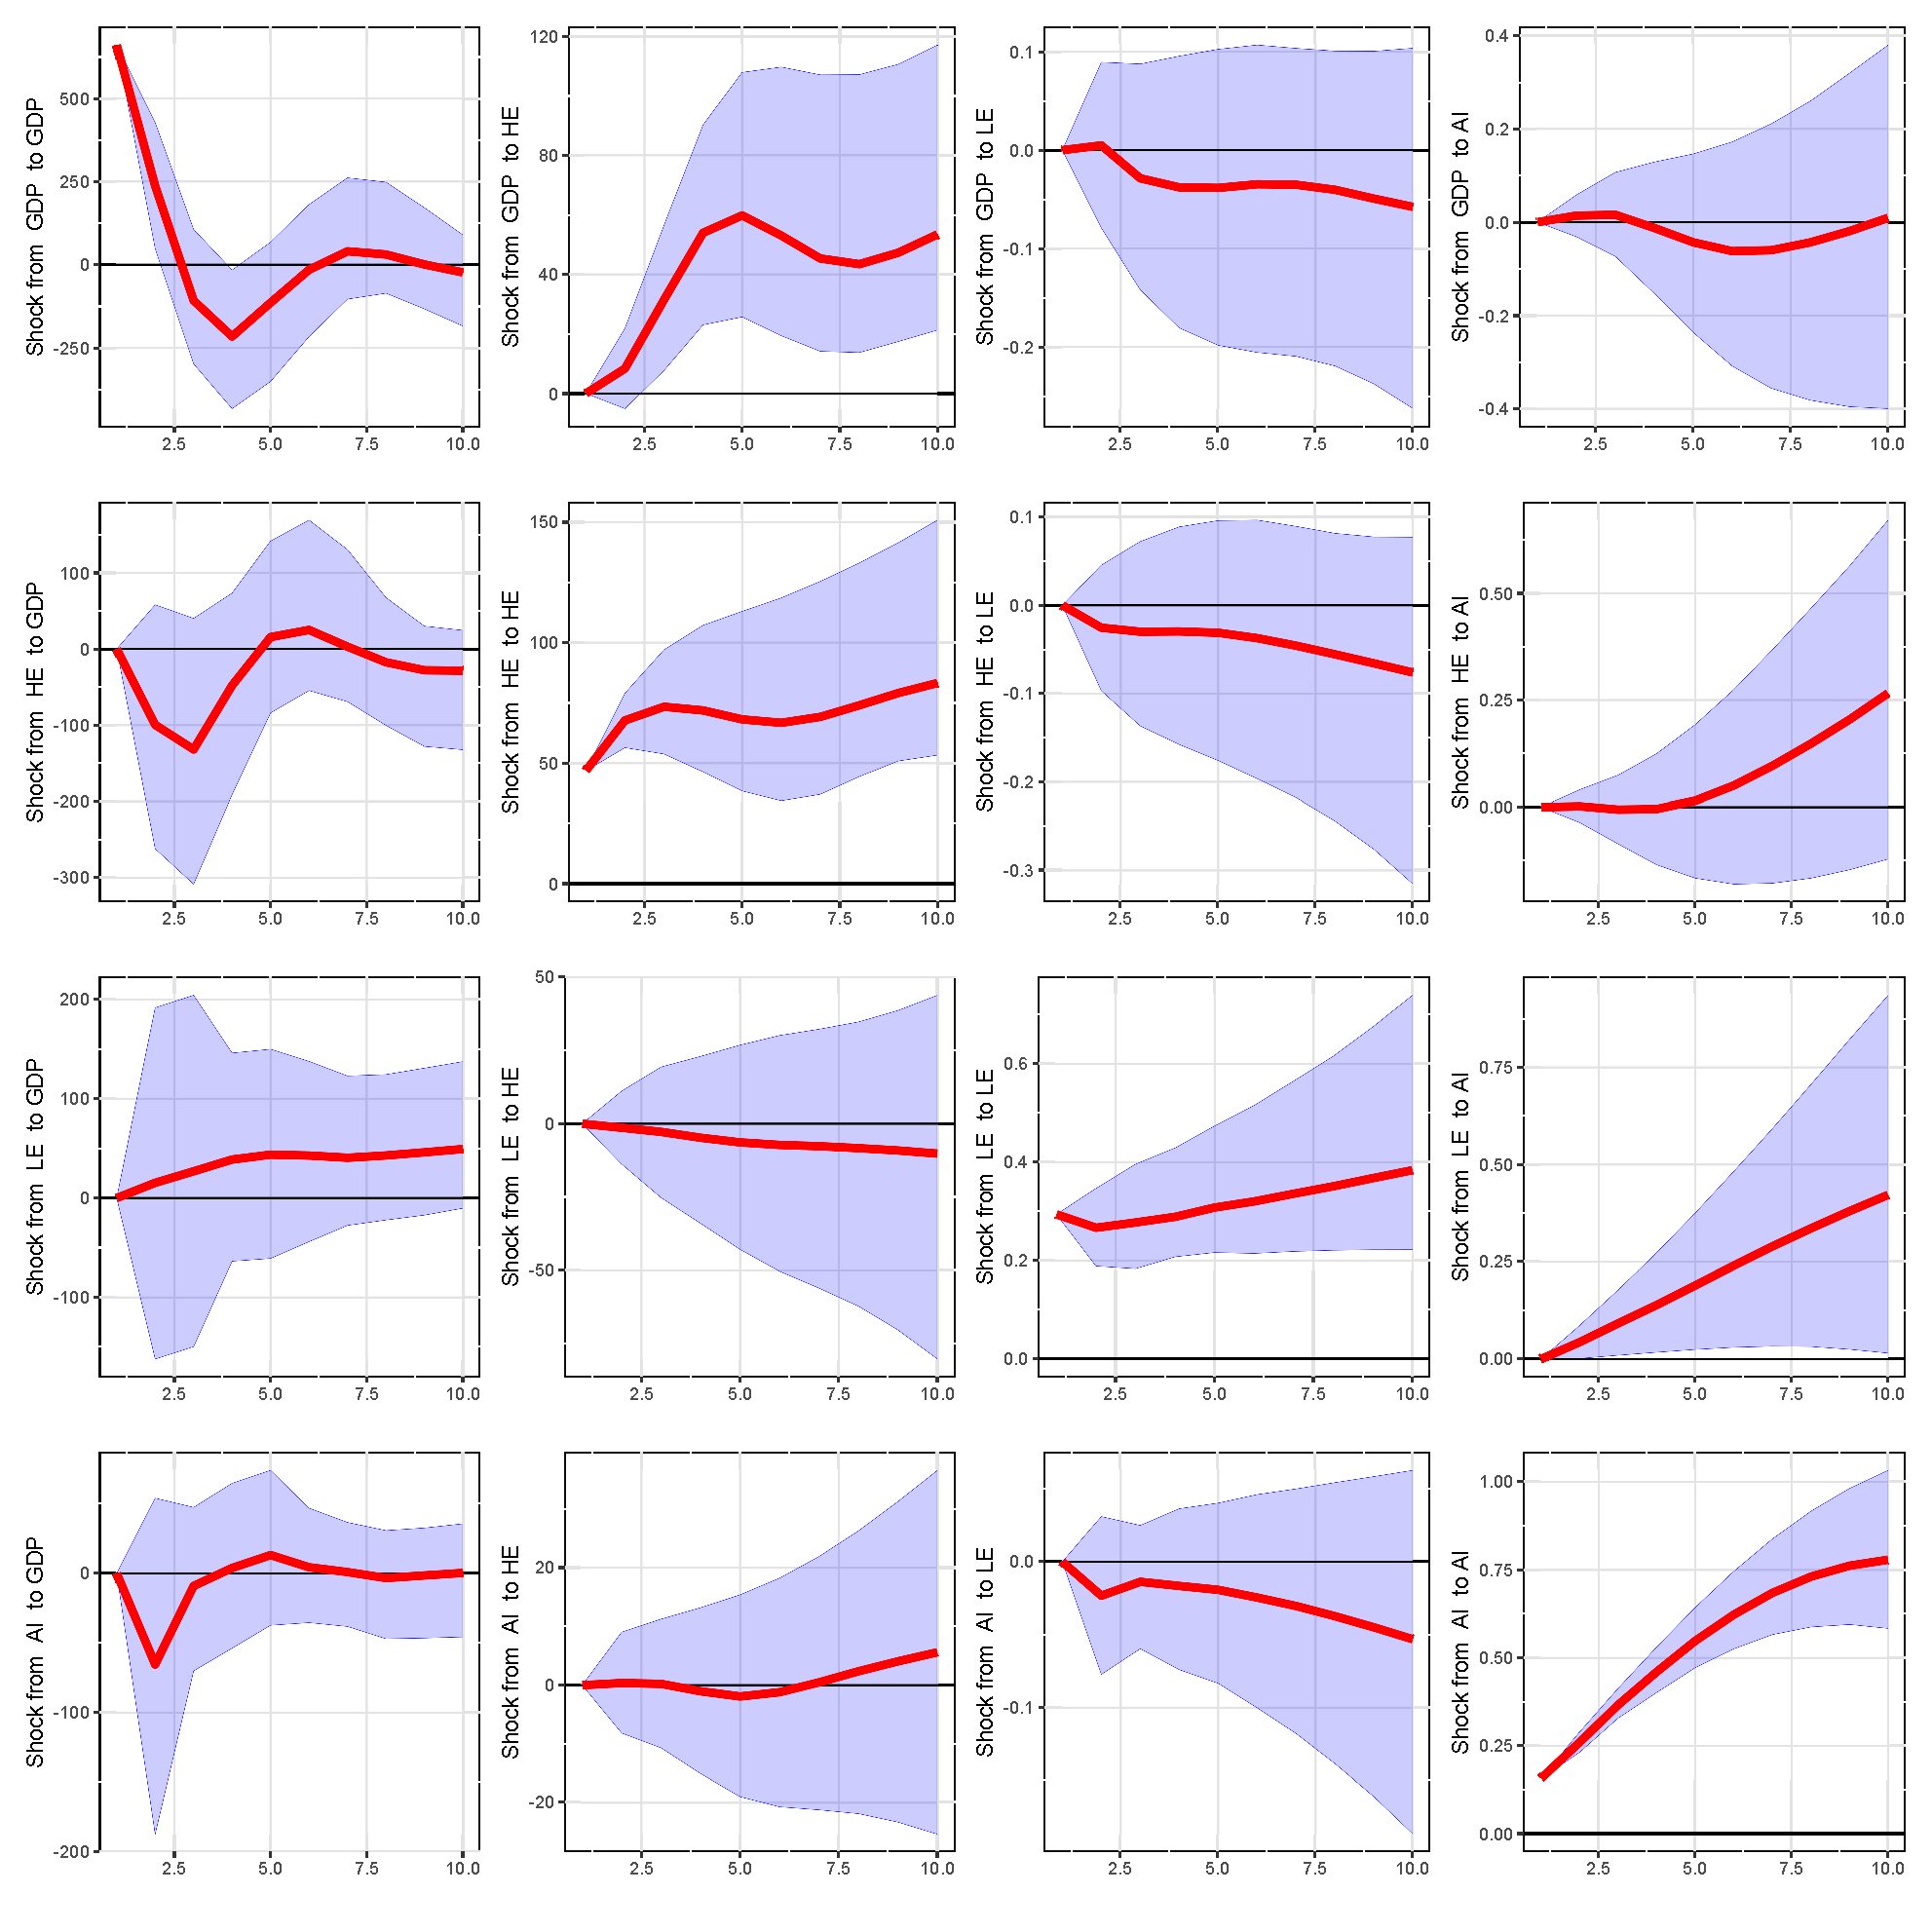
\includegraphics[width=\textwidth]{irf_minnesota.eps}
  \caption{Minnesota prior: Impulse responses. Each plot shows the percentage-point response of the indicated variable from its steady state to a one-standard-deviation indicated shock when the Minnesota prior was adopted. Periods are in years. In the case of responses from GDP (growth) and HE, the responses are given as the percentage point times 100.}
  \label{irf_minnesota}
\end{figure}

\begin{figure}
  \centering
  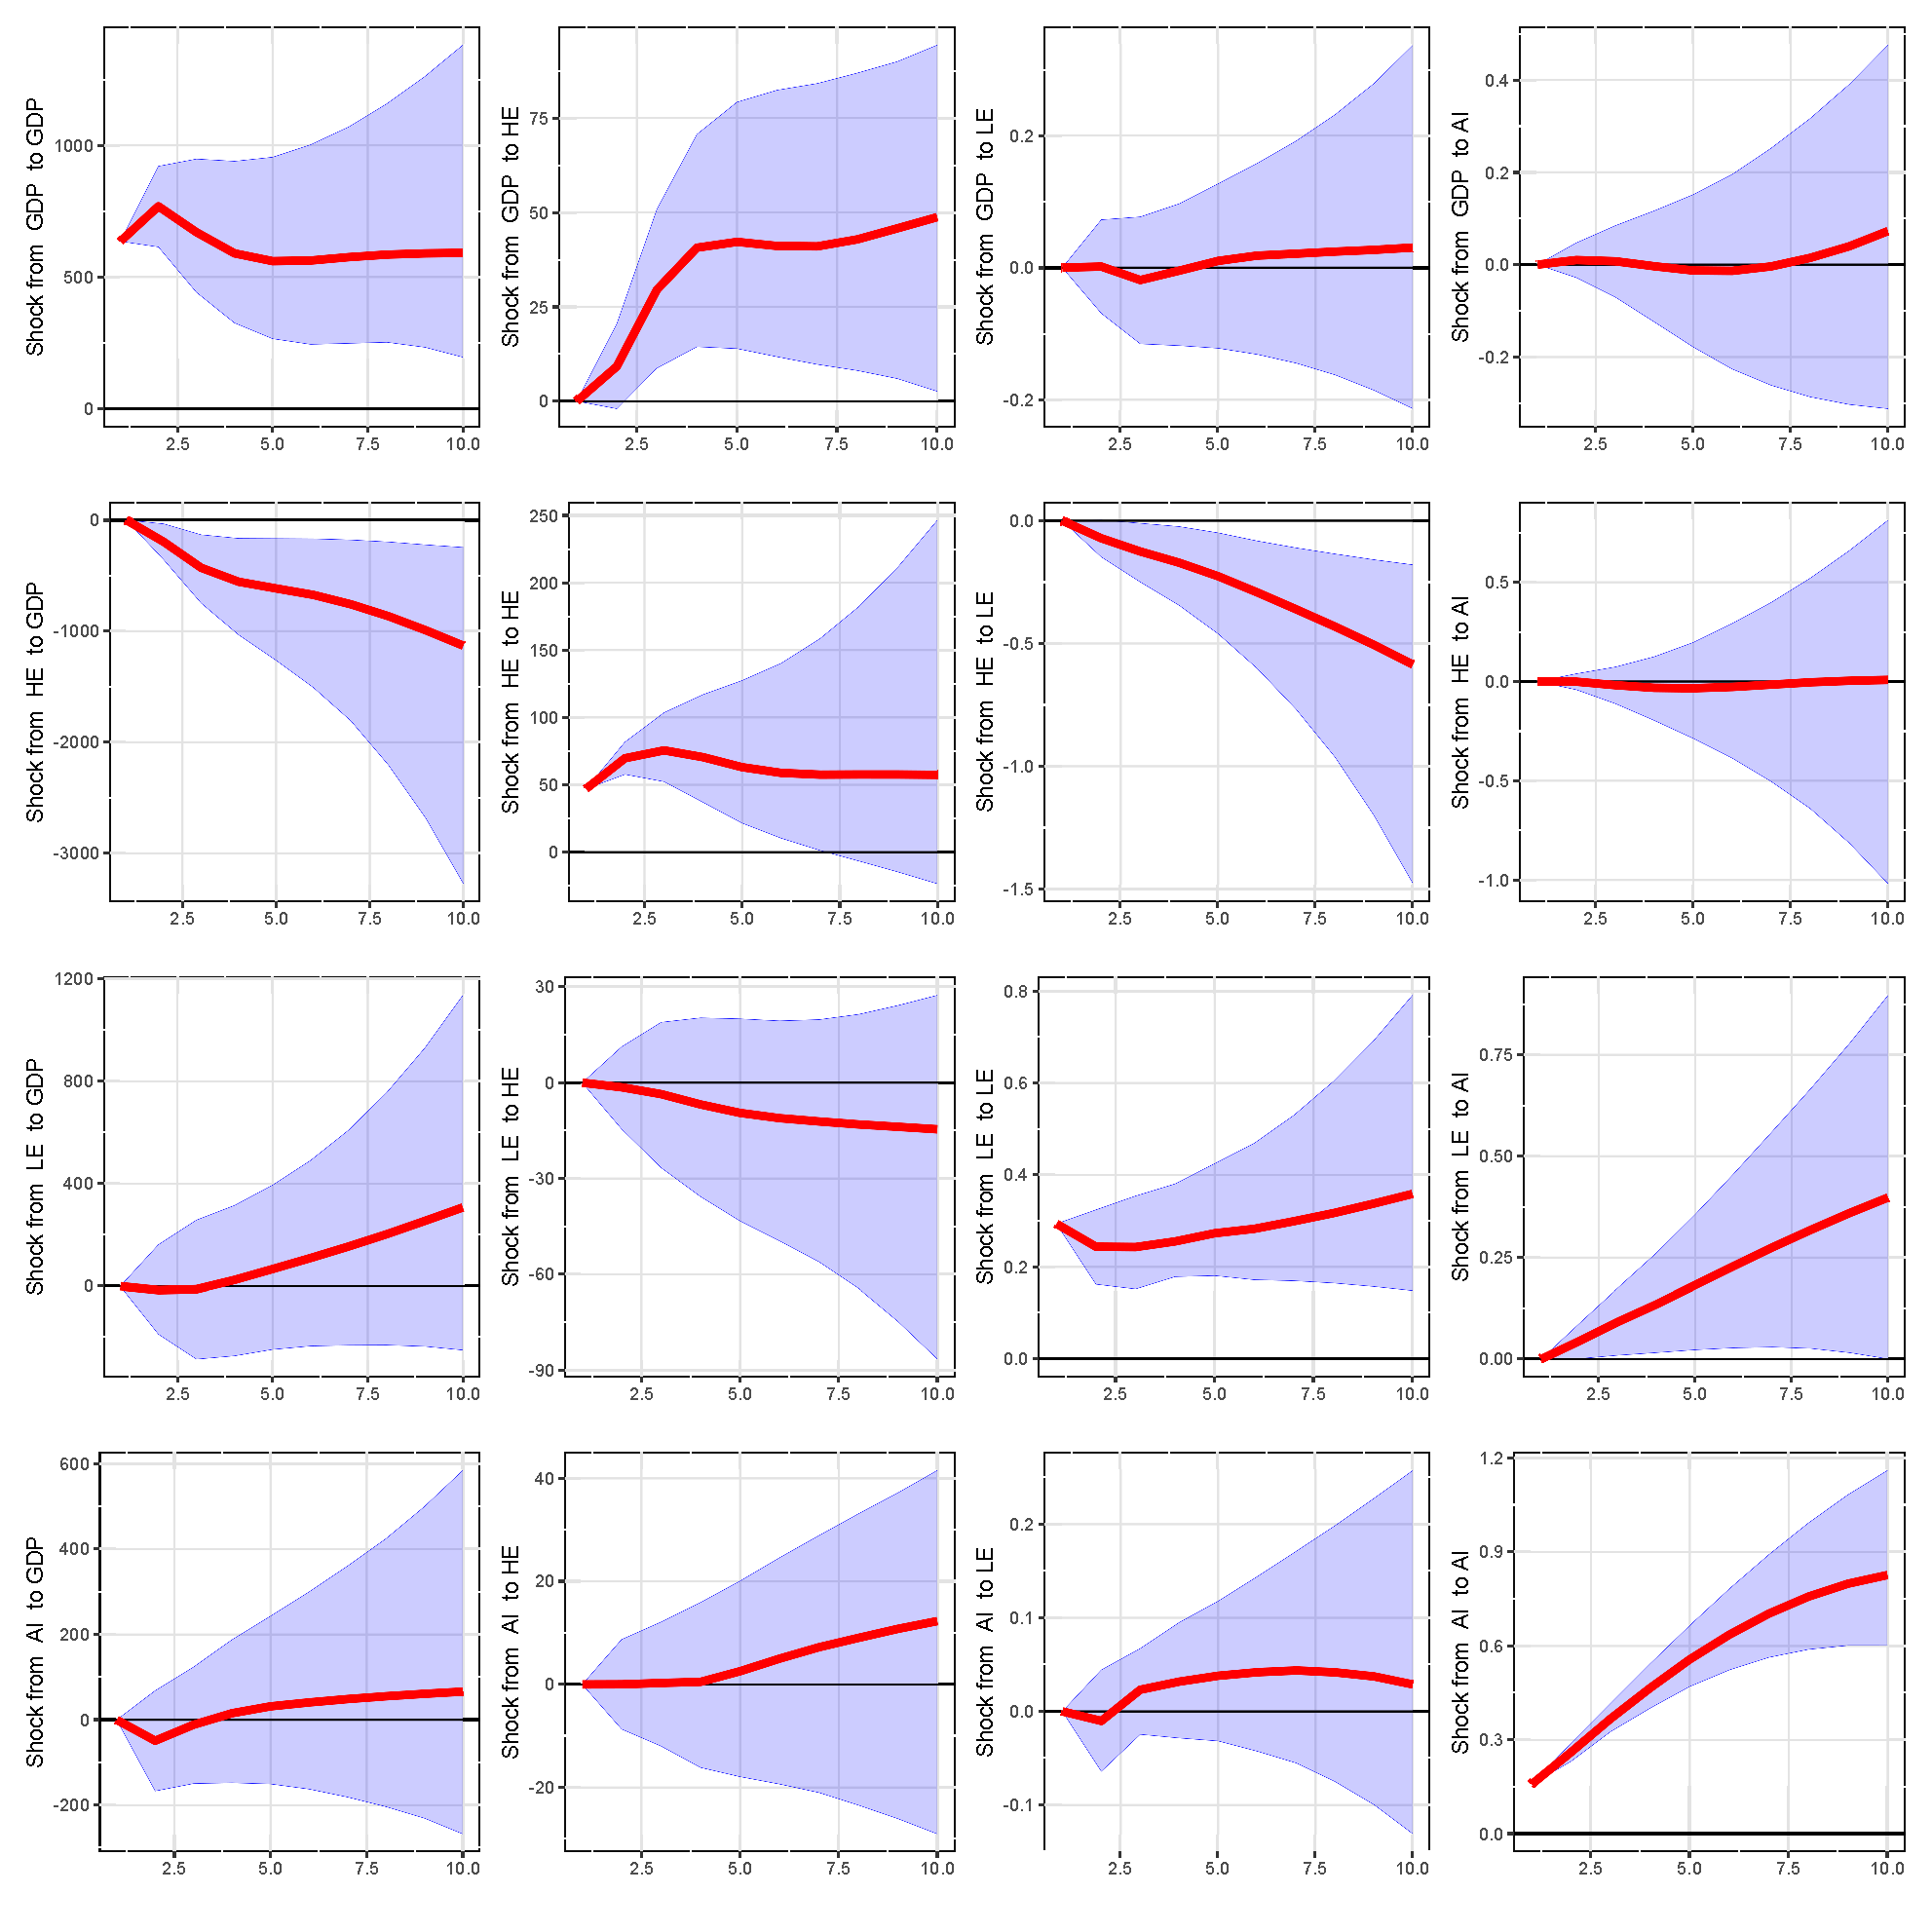
\includegraphics[width=\textwidth]{irf_iw.eps}
  \caption{Conditional normal inverse-Wishart prior: Impulse responses. Each plot shows the percentage-point response of the indicated variable from its steady state to a one-standard-deviation indicated shock when the Conditional normal inverse-Wishart  prior was adopted. Periods are in years. In the case of responses from GDP (growth) and HE, the responses are given as the percentage point times 100. }
  \label{irf_iw}
\end{figure}

\hypertarget{forecasts}{%
\subsection{Forecasts}\label{forecasts}}

The 20-year forecasts for the four variables under the adopted Minnesota
and conditional inverse-Wishart priors are shown in Figures
\ref{for_minnesota} and \ref{for_iw}, respectively. Due to the
similarities across Figures, I only analyse the case for the Minnesota
prior.

The projections show a persistent increase in the ageing index (AI) and
a continued decrease in life expectancy at birth (LE). This matches my
recent experience in the US and again highlights the source of the
reduced AI; the increased mortality of individuals aged 14 and younger
is larger than the lowered mortality for individuals aged 65 and over,
thereby reducing LE whilst increasing AI. As indicated in the impulse
response analysis, healthcare expenditure persistently increases due to
the lowered life expectancy.

\begin{figure}
  \centering
  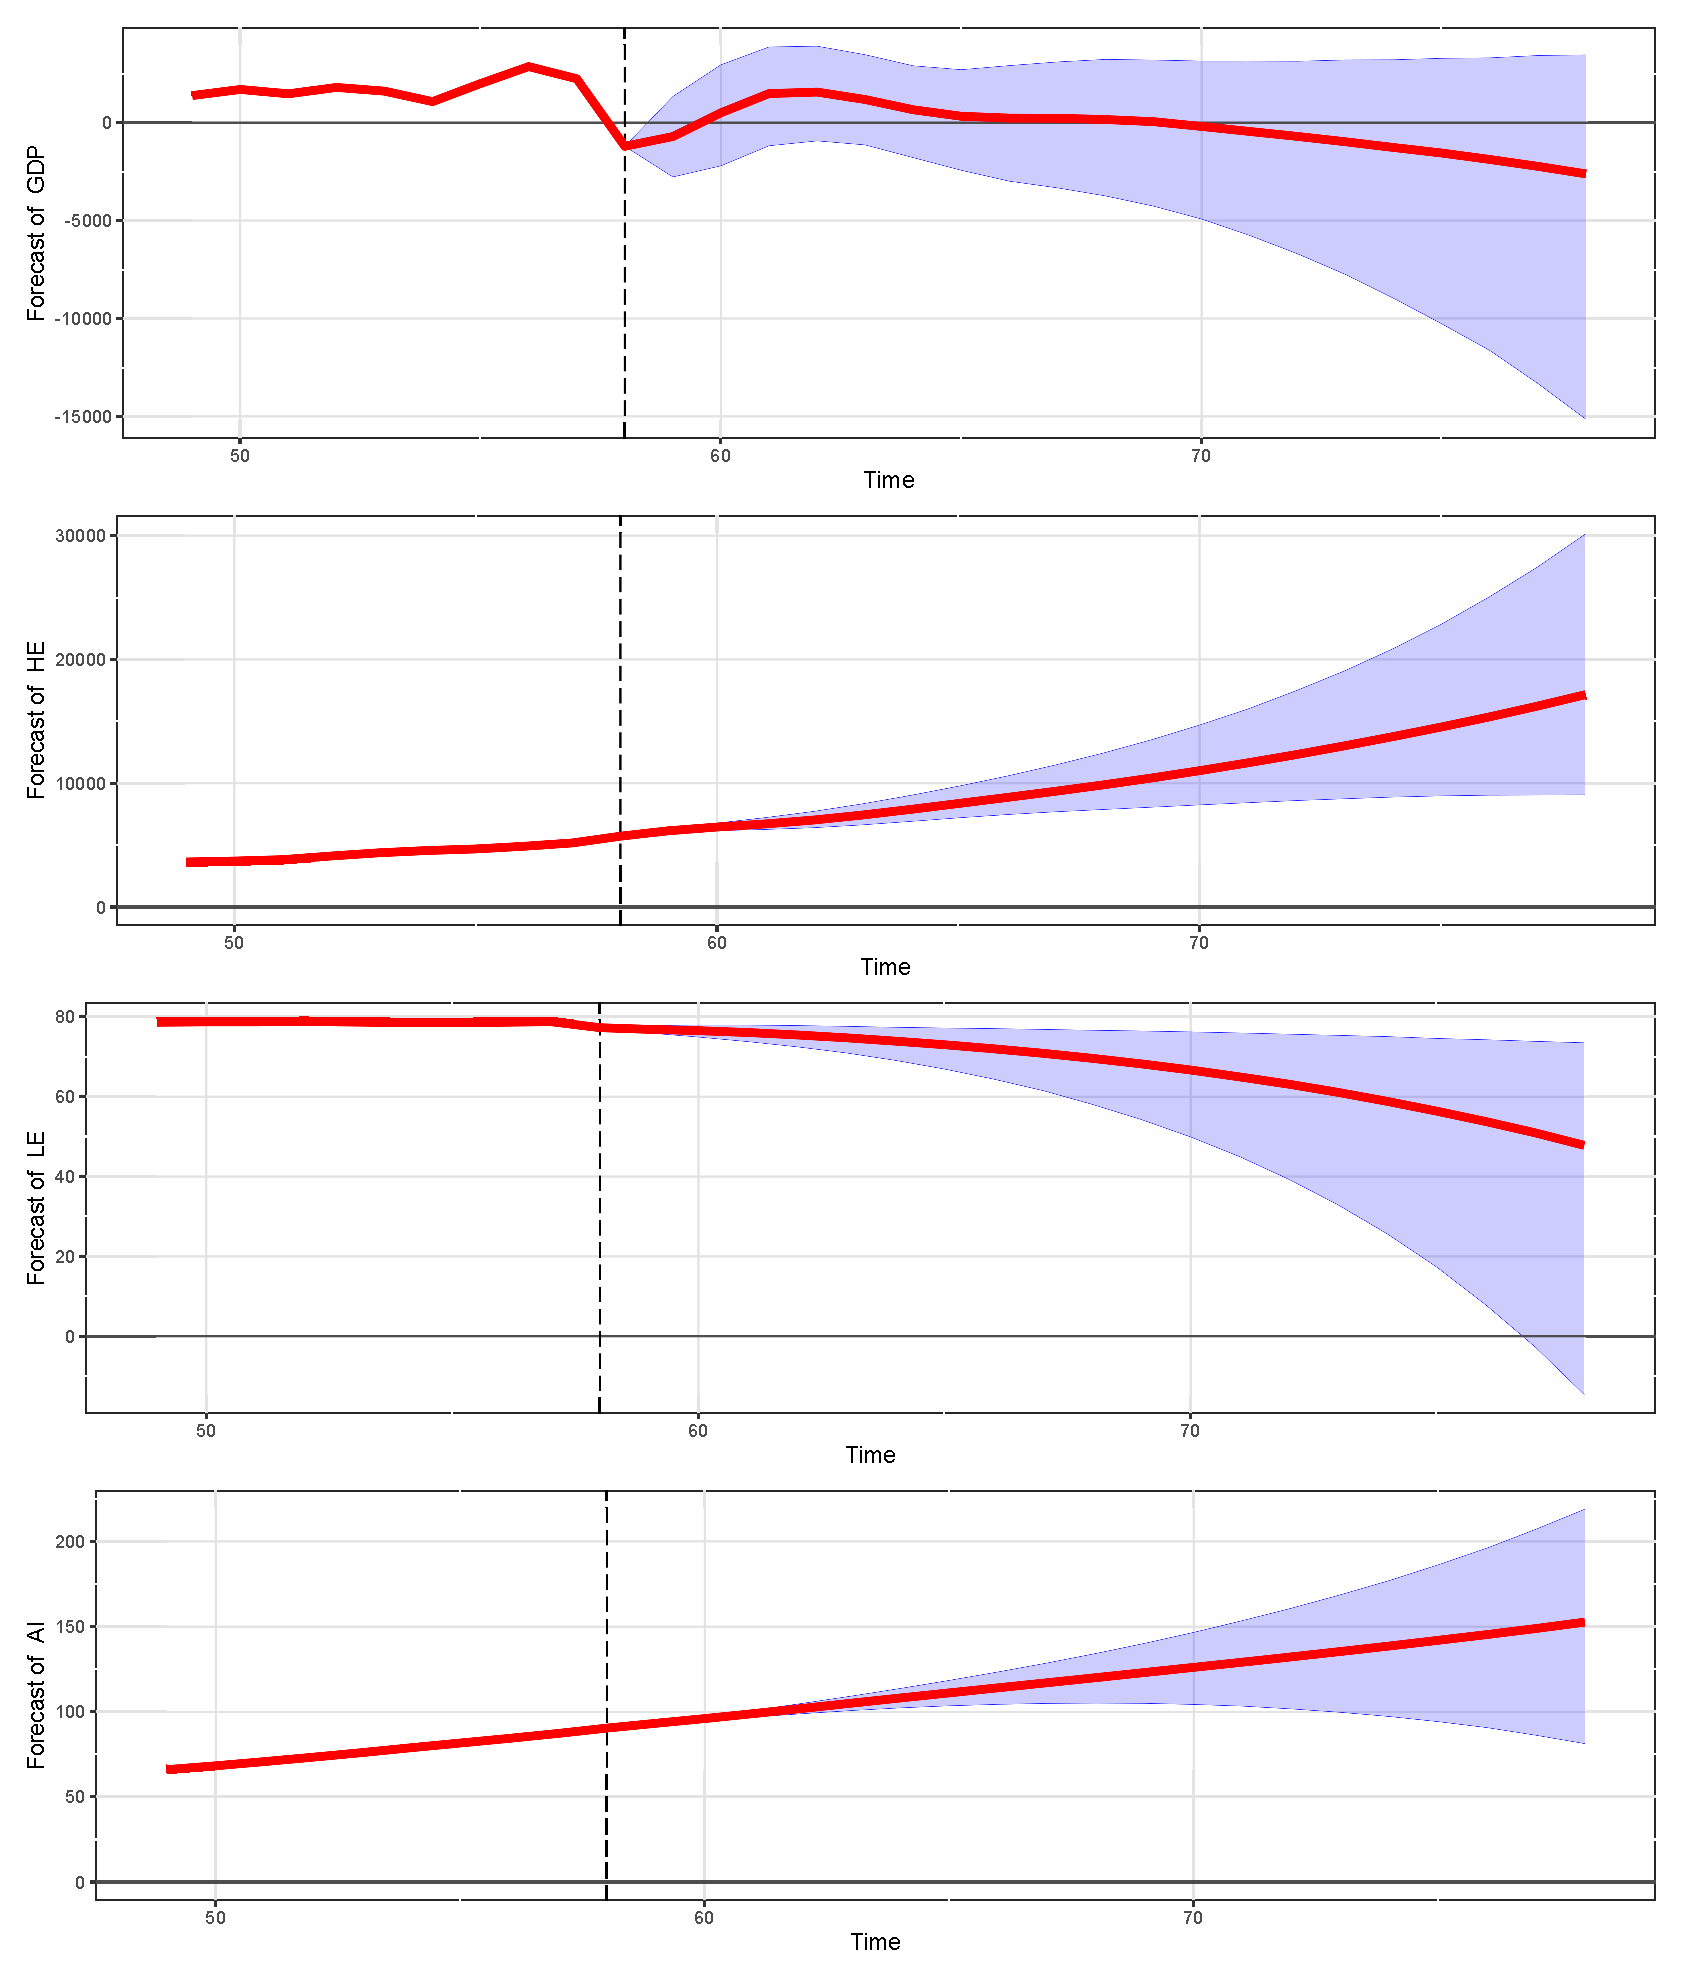
\includegraphics[width=\textwidth]{Forecast_minnesota.eps}
  \caption{Minnesota prior: Estimated forecasts. Periods are in years.}
  \label{for_minnesota}
\end{figure}

\begin{figure}
  \centering
  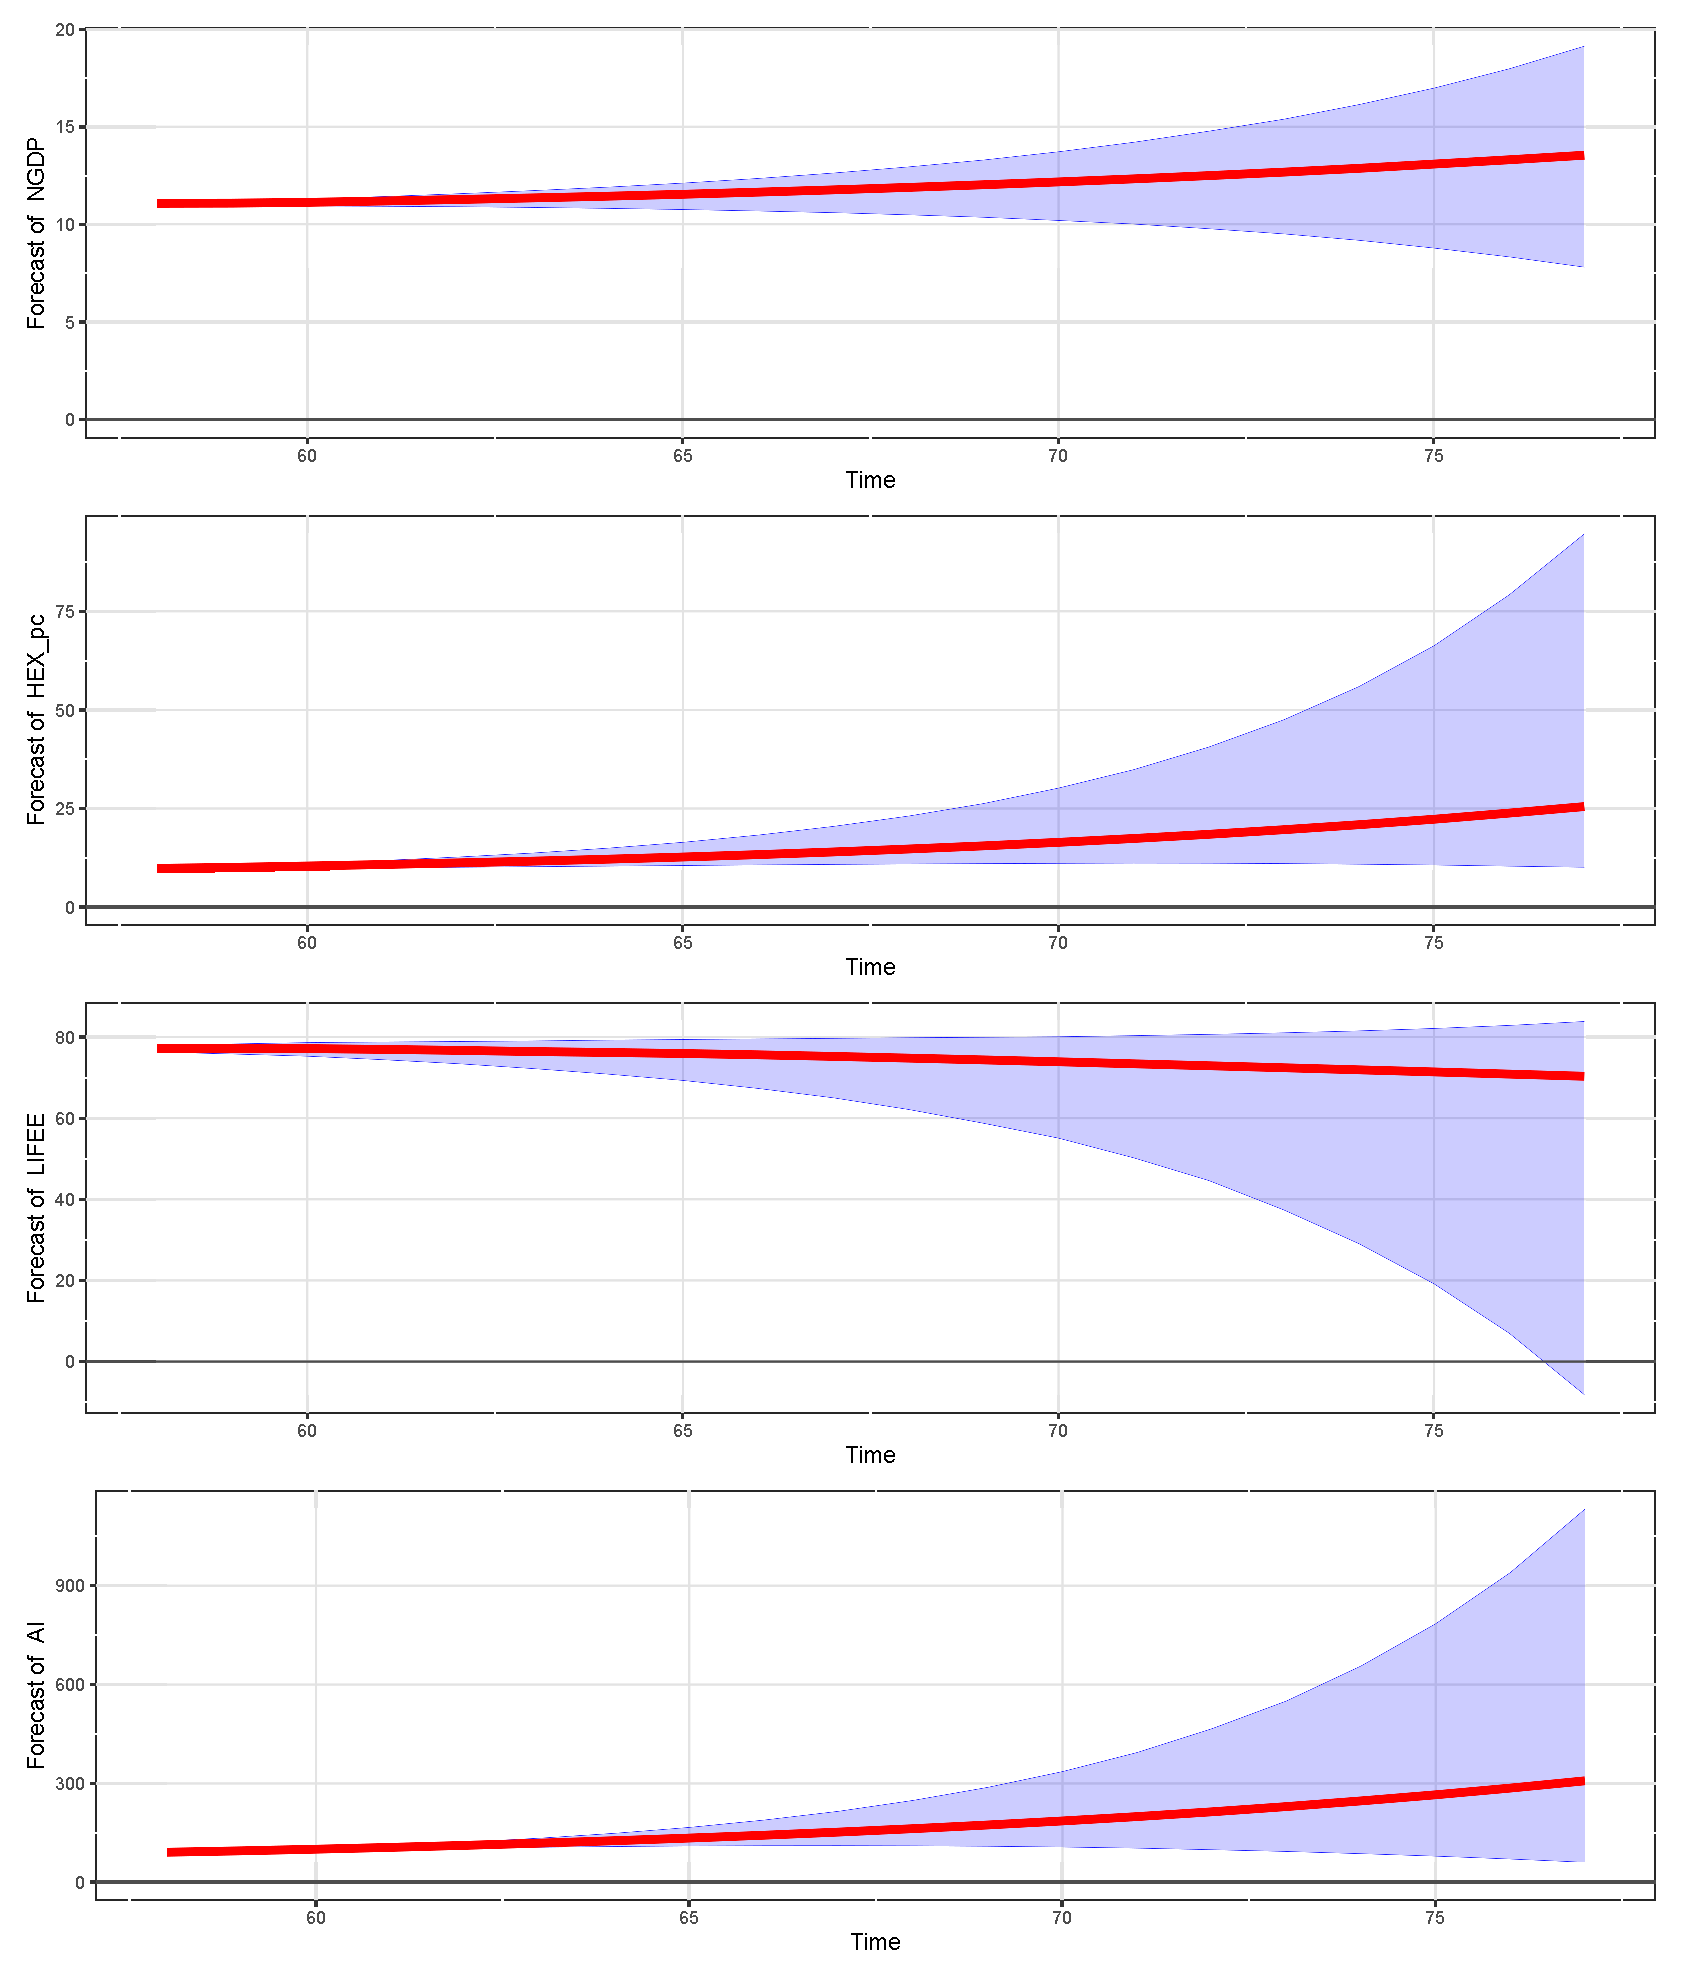
\includegraphics[width=\textwidth]{Forecast.eps}
  \caption{Conditional normal inverse-Wishart prior: Estimated forecasts. Periods are in years.}
  \label{for_iw}
\end{figure}

\hypertarget{references}{%
\section*{References}\label{references}}
\addcontentsline{toc}{section}{References}

\hypertarget{refs}{}
\begin{CSLReferences}{1}{0}
\leavevmode\vadjust pre{\hypertarget{ref-amiri2016}{}}%
Amiri, A. \& Linden, M. 2016. Income and total expenditure on health in
OECD countries: Evidence from panel data and hsiao's version of granger
non-causality tests. \emph{Economics and Business Letters}. 5(1):1--9.

\leavevmode\vadjust pre{\hypertarget{ref-amiri2012}{}}%
Amiri, A. \& Ventelou, B. 2012. Granger causality between total
expenditure on health and GDP in OECD: Evidence from the toda--yamamoto
approach. \emph{Economics letters}. 116(3):541--544.

\leavevmode\vadjust pre{\hypertarget{ref-baltagi2010}{}}%
Baltagi, B.H. \& Moscone, F. 2010. Health care expenditure and income in
the OECD reconsidered: Evidence from panel data. \emph{Economic
modelling}. 27(4):804--811.

\leavevmode\vadjust pre{\hypertarget{ref-bloom2010}{}}%
Bloom, D.E., Canning, D. \& Fink, G. 2010. Implications of population
ageing for economic growth. \emph{Oxford review of economic policy}.
26(4):583--612.

\leavevmode\vadjust pre{\hypertarget{ref-braendle2016}{}}%
Braendle, T. \& Colombier, C. 2016. What drives public health care
expenditure growth? Evidence from swiss cantons, 1970--2012.
\emph{Health Policy}. 120(9):1051--1060.

\leavevmode\vadjust pre{\hypertarget{ref-canova2007}{}}%
Canova, F. 2007. \emph{Methods for applied macroeconomic research}. Vol.
13. Princeton university press.

\leavevmode\vadjust pre{\hypertarget{ref-chaabouni2016}{}}%
Chaabouni, S., Zghidi, N. \& Mbarek, M.B. 2016. On the causal dynamics
between CO2 emissions, health expenditures and economic growth.
\emph{Sustainable cities and society}. 22:184--191.

\leavevmode\vadjust pre{\hypertarget{ref-chan2017notes}{}}%
Chan, J.C. 2017. Notes on bayesian macroeconometrics. \emph{Manuscript
available at http://joshuachan. org}.

\leavevmode\vadjust pre{\hypertarget{ref-cheng2020}{}}%
Cheng, X., Yang, Y., Schwebel, D.C., Liu, Z., Li, L., Cheng, P., Ning,
P. \& Hu, G. 2020. Population ageing and mortality during 1990--2017: A
global decomposition analysis. \emph{PLoS medicine}. 17(6):e1003138.

\leavevmode\vadjust pre{\hypertarget{ref-dickey1979}{}}%
Dickey, D.A. \& Fuller, W.A. 1979. Distribution of the estimators for
autoregressive time series with a unit root. \emph{Journal of the
American statistical association}. 74(366a):427--431.

\leavevmode\vadjust pre{\hypertarget{ref-doan1984}{}}%
Doan, T., Litterman, R. \& Sims, C. 1984. Forecasting and conditional
projection using realistic prior distributions. \emph{Econometric
reviews}. 3(1):1--100.

\leavevmode\vadjust pre{\hypertarget{ref-fogel2004}{}}%
Fogel, R.W. 2004. Health, nutrition, and economic growth. \emph{Economic
development and cultural change}. 52(3):643--658.

\leavevmode\vadjust pre{\hypertarget{ref-halici2016}{}}%
Halıcı-Tülüce, N.S., Doğan, İ. \& Dumrul, C. 2016. Is income relevant
for health expenditure and economic growth nexus? \emph{International
journal of health economics and management}. 16:23--49.

\leavevmode\vadjust pre{\hypertarget{ref-jaba2014}{}}%
Jaba, E., Balan, C.B. \& Robu, I.-B. 2014. The relationship between life
expectancy at birth and health expenditures estimated by a cross-country
and time-series analysis. \emph{Procedia Economics and Finance}.
15:108--114.

\leavevmode\vadjust pre{\hypertarget{ref-koop2010}{}}%
Koop, G. \& Korobilis, D. 2010. Bayesian multivariate time series
methods for empirical macroeconomics. \emph{Foundations and
Trends{\textregistered} in Econometrics}. 3(4):267--358.

\leavevmode\vadjust pre{\hypertarget{ref-lee2000}{}}%
Lee, R., Mason, A. \& Miller, T. 2000. Life cycle saving and the
demographic transition: The case of taiwan. \emph{Population and
Development Review}. 26:194--219.

\leavevmode\vadjust pre{\hypertarget{ref-linden2017}{}}%
Linden, M. \& Ray, D. 2017. Life expectancy effects of public and
private health expenditures in OECD countries 1970--2012: Panel time
series approach. \emph{Economic Analysis and Policy}. 56:101--113.

\leavevmode\vadjust pre{\hypertarget{ref-liotta2018}{}}%
Liotta, G., Canhao, H., Cenko, F., Cutini, R., Vellone, E., Illario, M.,
Kardas, P., Poscia, A., et al. 2018. Active ageing in europe: Adding
healthy life to years. \emph{Frontiers in medicine}. 5:123.

\leavevmode\vadjust pre{\hypertarget{ref-litterman1986}{}}%
Litterman, R.B. 1986. Forecasting with bayesian vector
autoregressions---five years of experience. \emph{Journal of Business \&
Economic Statistics}. 4(1):25--38.

\leavevmode\vadjust pre{\hypertarget{ref-lopreite2017}{}}%
Lopreite, M. \& Mauro, M. 2017. The effects of population ageing on
health care expenditure: A bayesian VAR analysis using data from italy.
\emph{Health policy}. 121(6):663--674.

\leavevmode\vadjust pre{\hypertarget{ref-lopreite2020}{}}%
Lopreite, M. \& Zhu, Z. 2020. The effects of ageing population on health
expenditure and economic growth in china: A bayesian-VAR approach.
\emph{Social science \& medicine}. 265:113513.

\leavevmode\vadjust pre{\hypertarget{ref-murillo1993}{}}%
Murillo, C., Piatecki, C. \& Saez, M. 1993. Health care expenditure and
income in europe. \emph{Health Economics}. 2(2):127--138.

\leavevmode\vadjust pre{\hypertarget{ref-murthy2016}{}}%
Murthy, V.N. \& Okunade, A.A. 2016. Determinants of US health
expenditure: Evidence from autoregressive distributed lag (ARDL)
approach to cointegration. \emph{Economic Modelling}. 59:67--73.

\leavevmode\vadjust pre{\hypertarget{ref-wang2011}{}}%
Wang, K.-M. 2011. Health care expenditure and economic growth: Quantile
panel-type analysis. \emph{Economic modelling}. 28(4):1536--1549.

\leavevmode\vadjust pre{\hypertarget{ref-wiener2002}{}}%
Wiener, J.M. \& Tilly, J. 2002. Population ageing in the united states
of america: Implications for public programmes. \emph{International
journal of epidemiology}. 31(4):776--781.

\leavevmode\vadjust pre{\hypertarget{ref-williams2019}{}}%
Williams, G., Cylus, J., Roubal, T., Ong, P., Barber, S., Organization,
W.H., et al. 2019. Sustainable health financing with an ageing
population: Will population ageing lead to uncontrolled health
expenditure growth?

\end{CSLReferences}

\newpage
\appendix
\renewcommand{\thesection}{Appendix A}

\hypertarget{section}{%
\section{\texorpdfstring{\label{aa}}{}}\label{section}}

\begin{figure}
     \centering
     \begin{subfigure}[H]{0.49\textwidth}
         \centering
         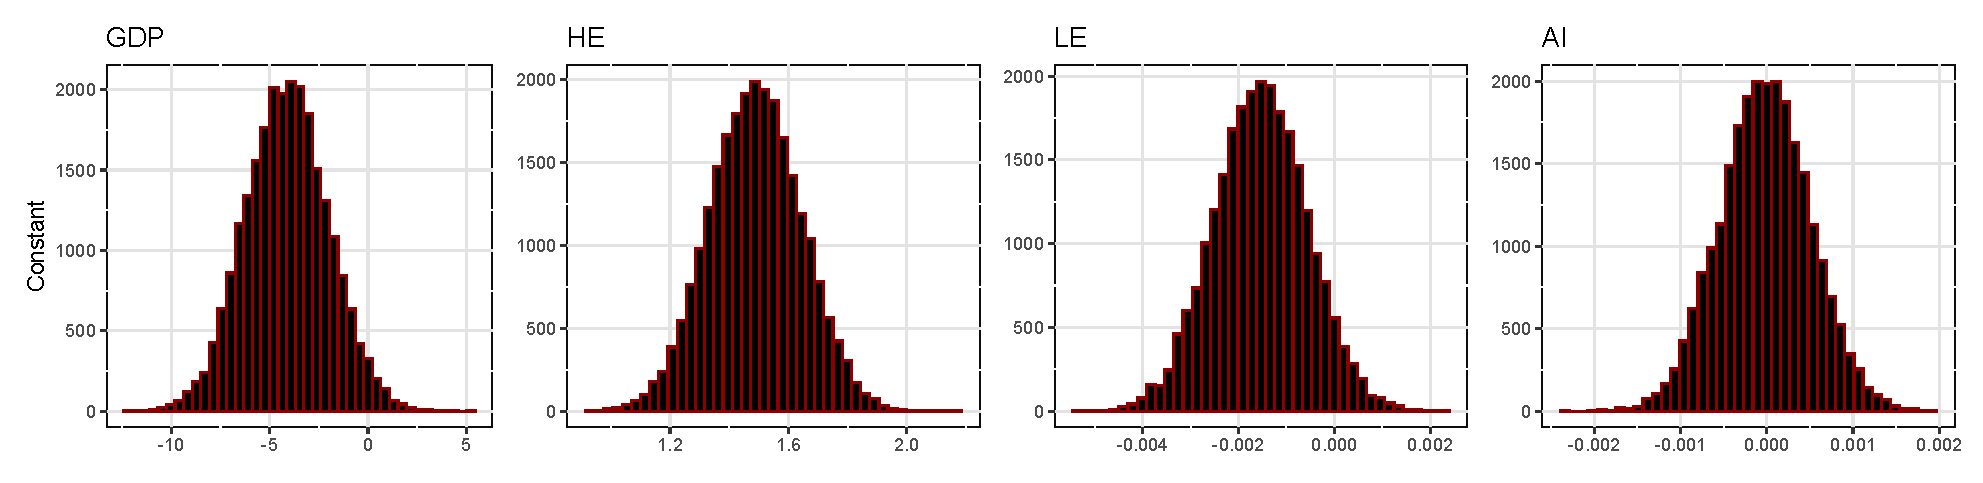
\includegraphics[width=\textwidth]{minn_Constant.eps}
     \end{subfigure}
     \begin{subfigure}[H]{0.49\textwidth}
         \centering
         \includegraphics[width=\textwidth]{minn_CoefLag1.eps}
     \end{subfigure}
    \begin{subfigure}[H]{0.49\textwidth}
         \centering
         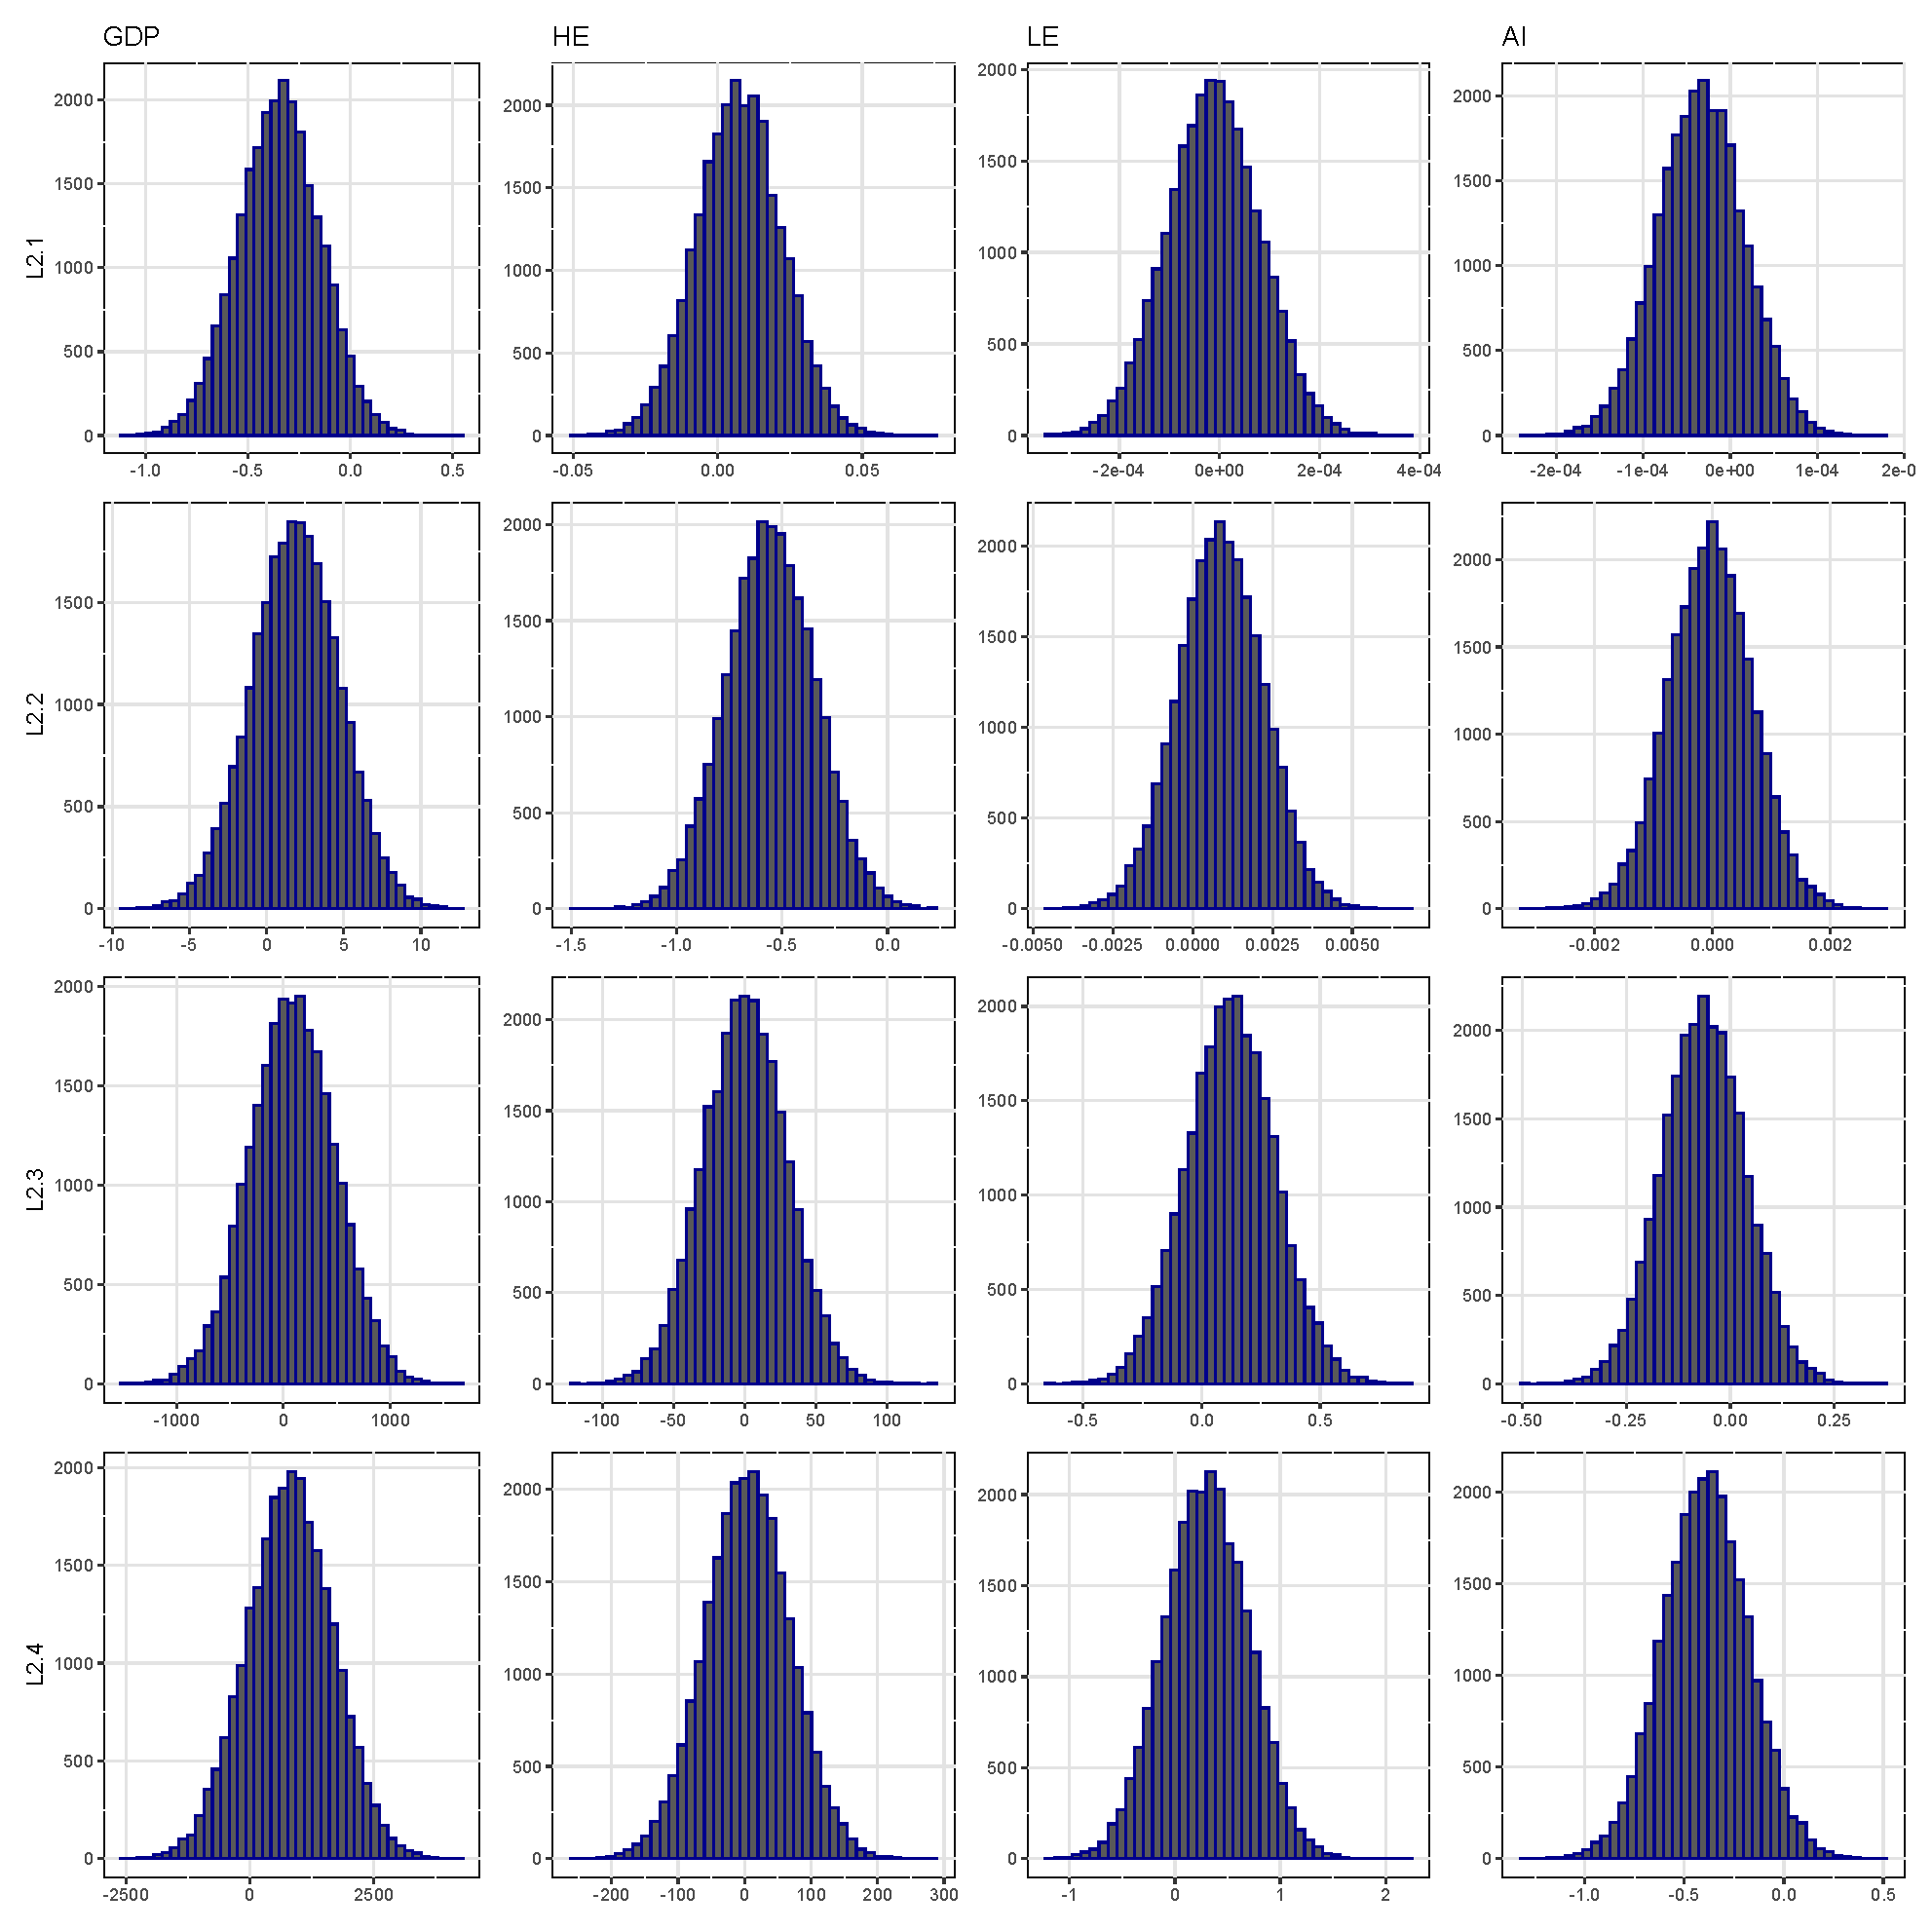
\includegraphics[width=\textwidth]{minn_CoefLag2.eps}
     \end{subfigure}
    \begin{subfigure}[H]{0.49\textwidth}
         \centering
         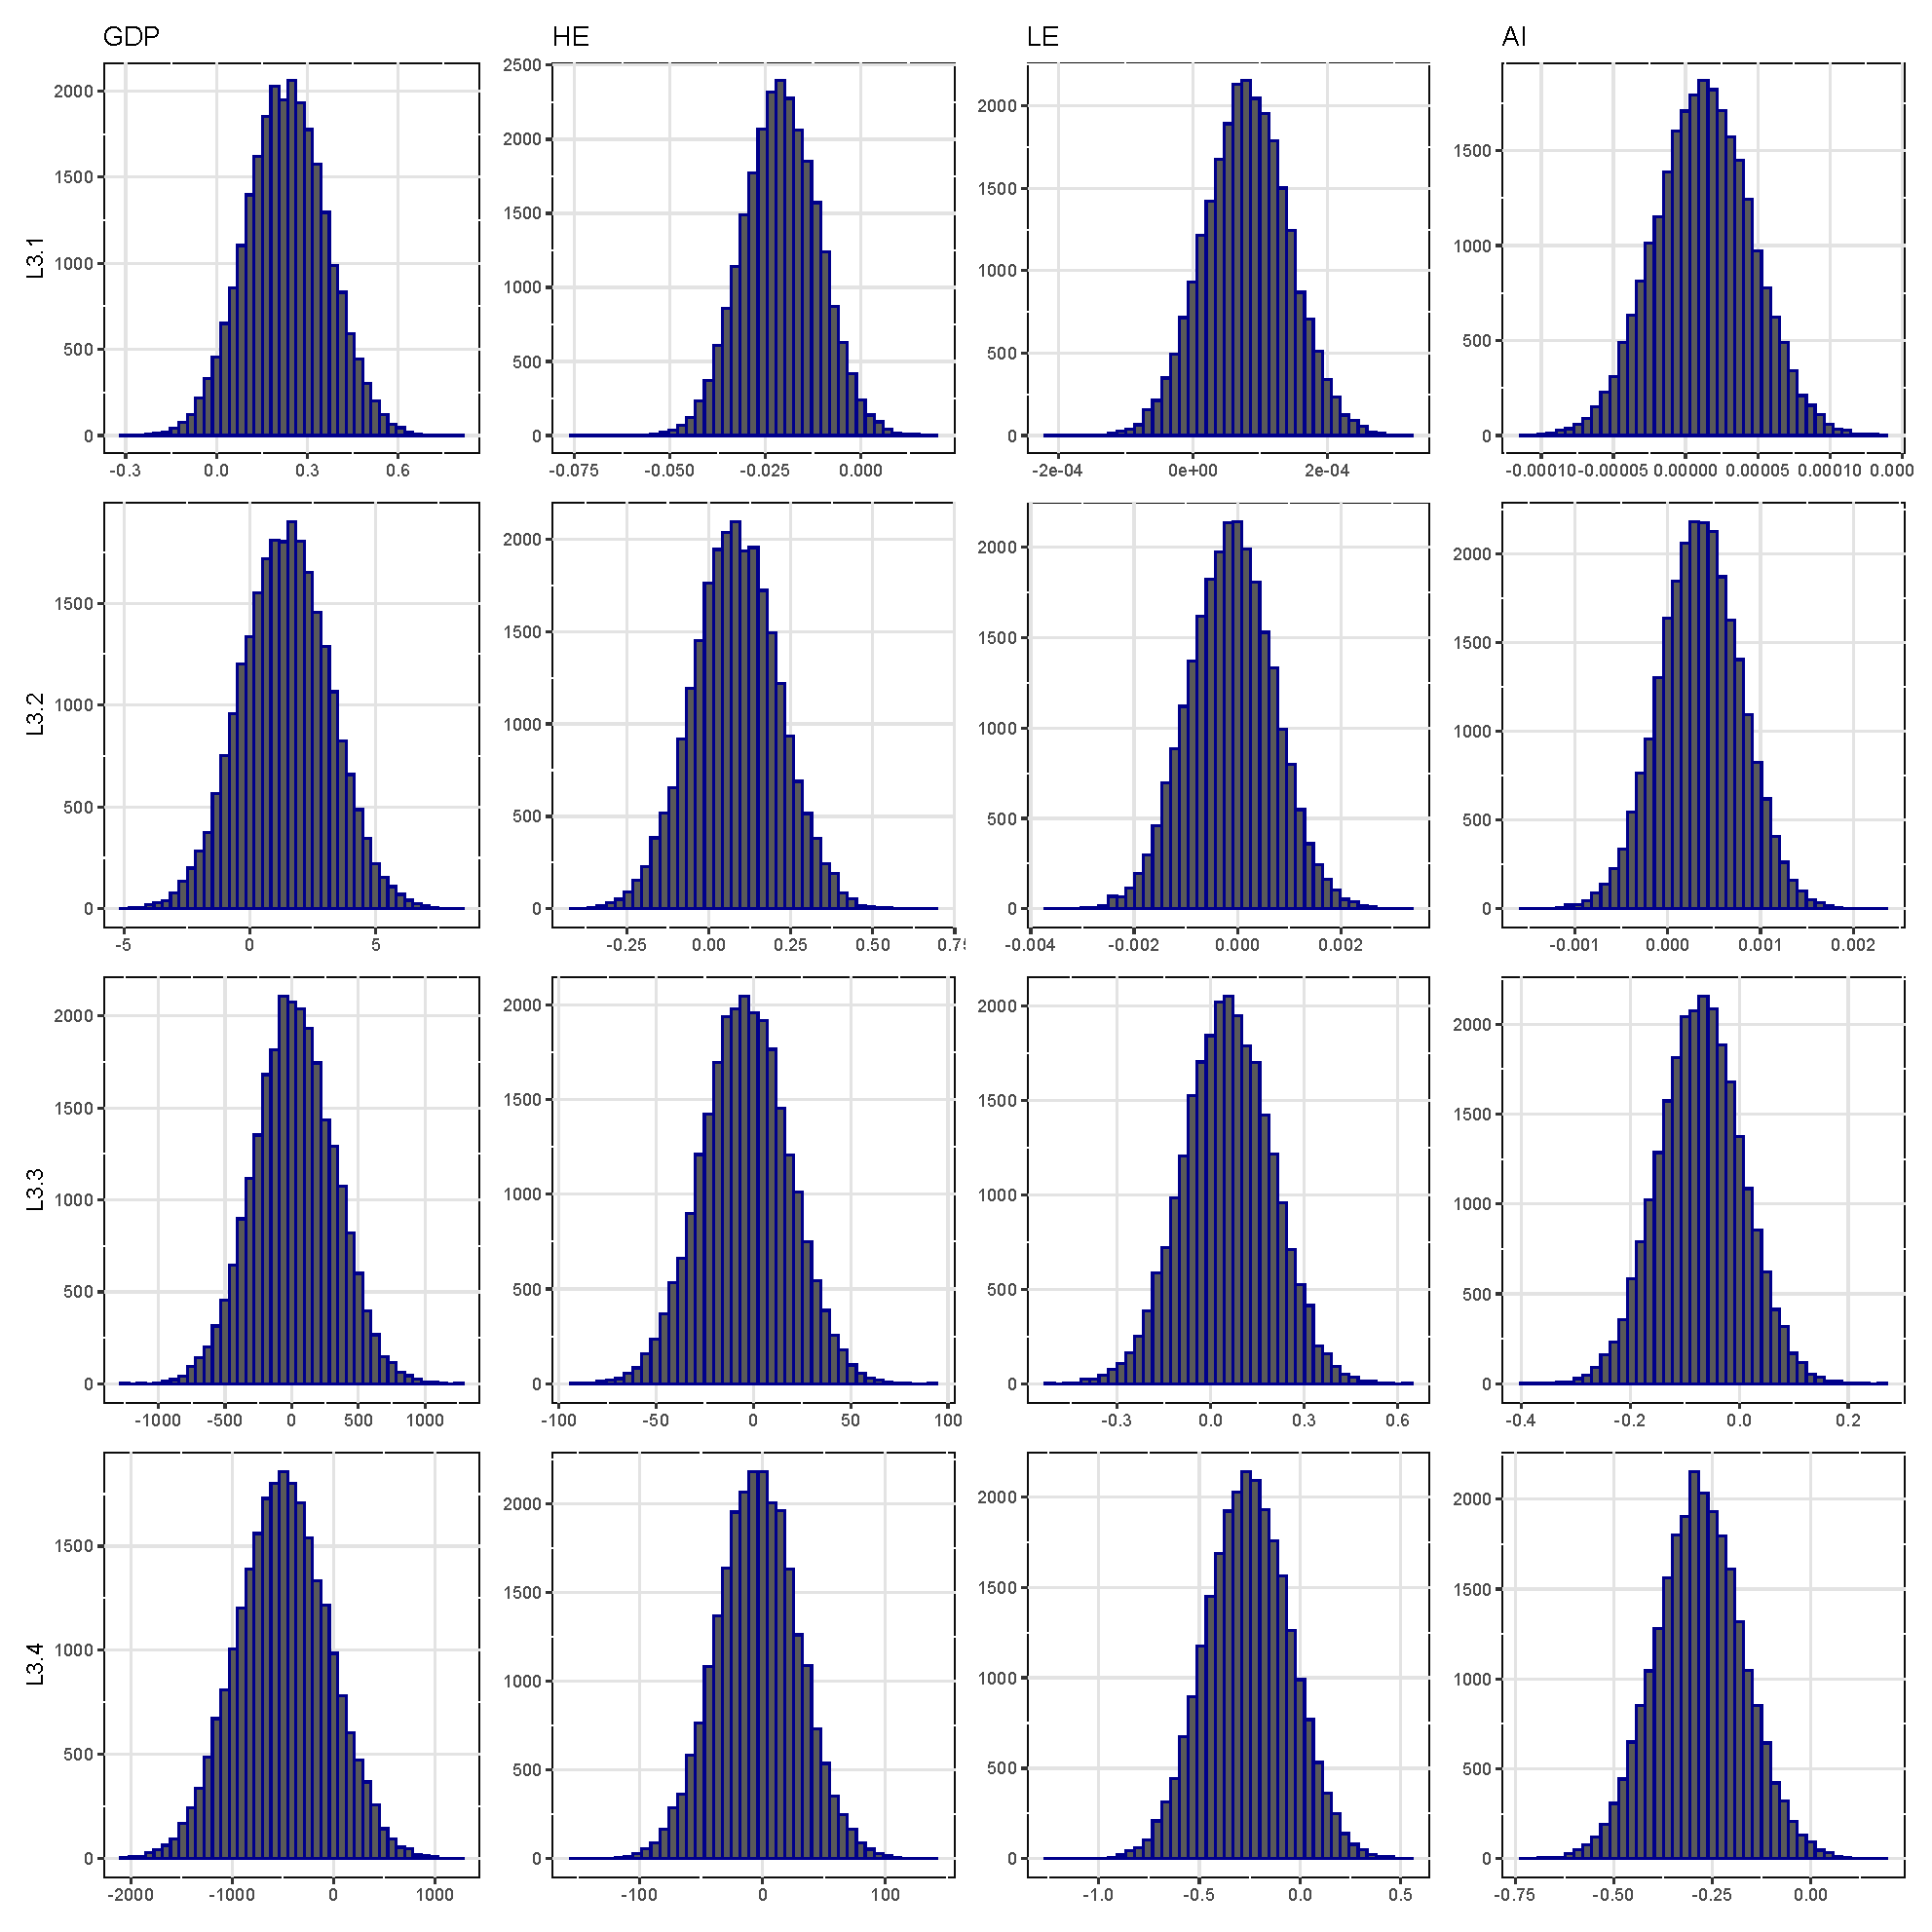
\includegraphics[width=\textwidth]{minn_CoefLag3.eps}
    \end{subfigure}
        \caption{Minnesota prior: Estimated BVAR(3) coefficients' posterior distributions using Gibbs sampling.}
        \label{posterior_minnesota}
\end{figure}

\begin{figure}
     \centering
     \begin{subfigure}[H]{0.49\textwidth}
         \centering
         \includegraphics[width=\textwidth]{Constant.eps}
     \end{subfigure}
     \begin{subfigure}[H]{0.49\textwidth}
         \centering
         \includegraphics[width=\textwidth]{CoefLag1.eps}
     \end{subfigure}
    \begin{subfigure}[H]{0.49\textwidth}
         \centering
         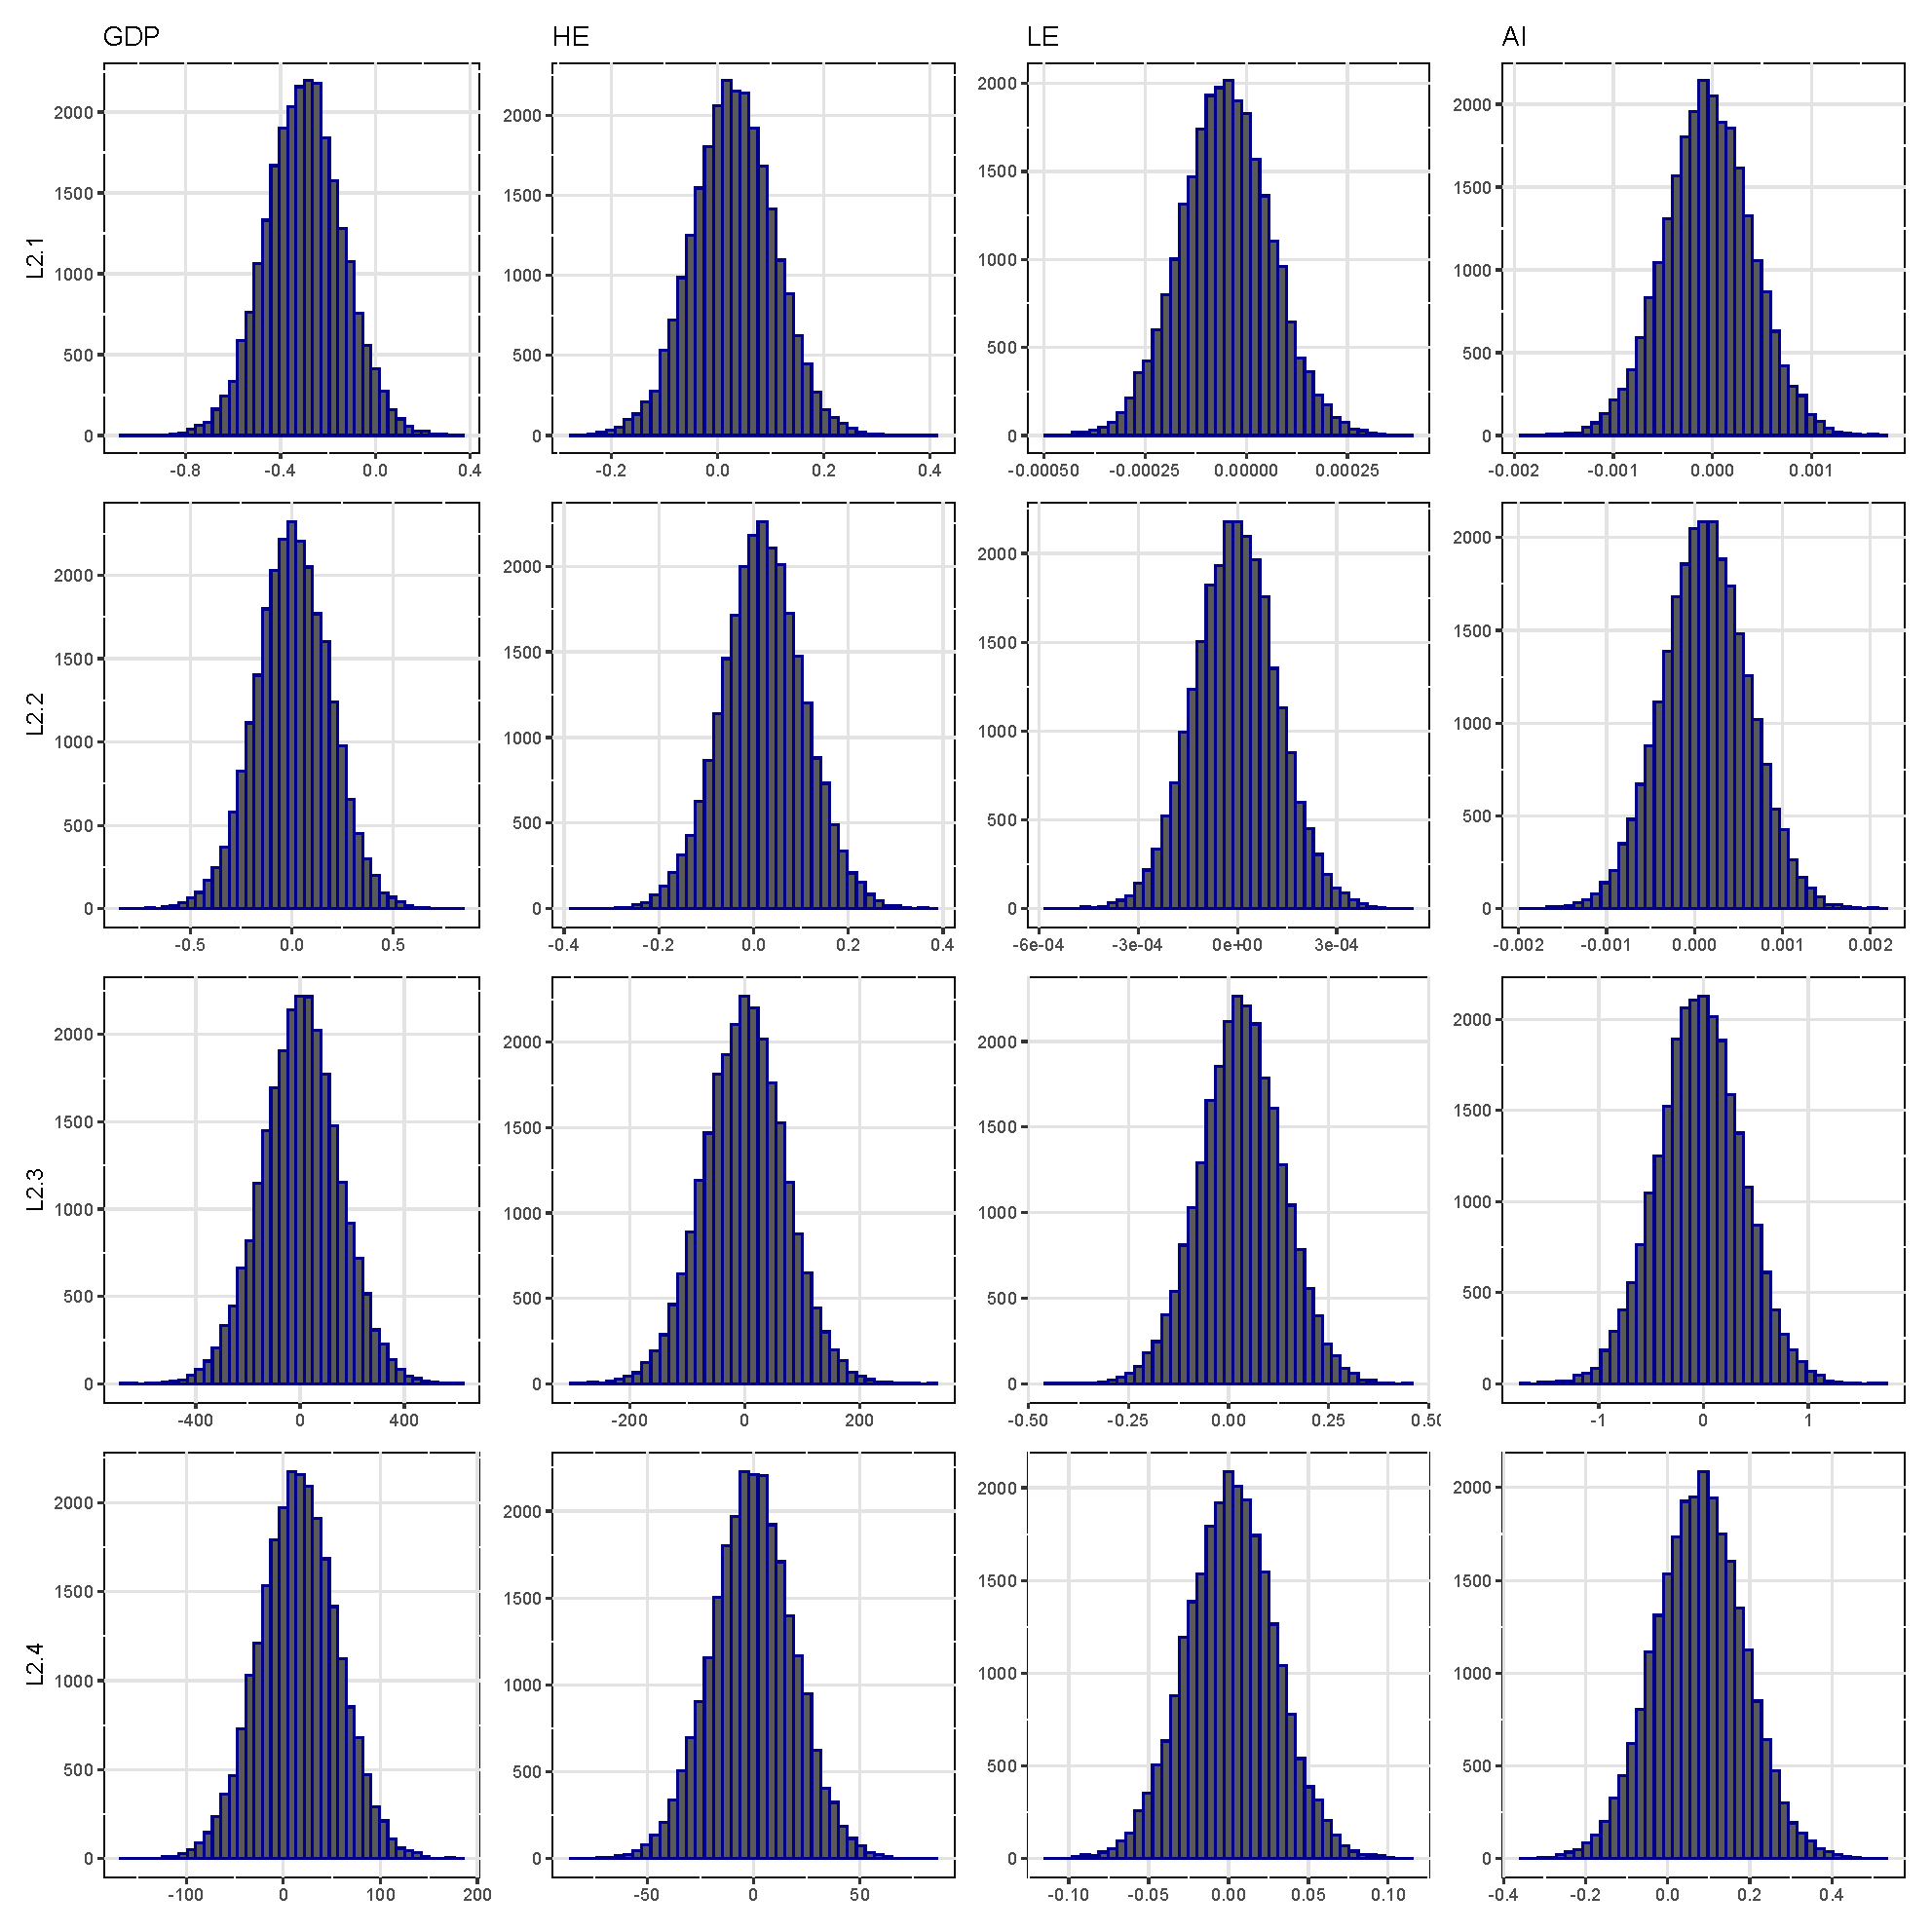
\includegraphics[width=\textwidth]{CoefLag2.eps}
     \end{subfigure}
    \begin{subfigure}[H]{0.49\textwidth}
         \centering
         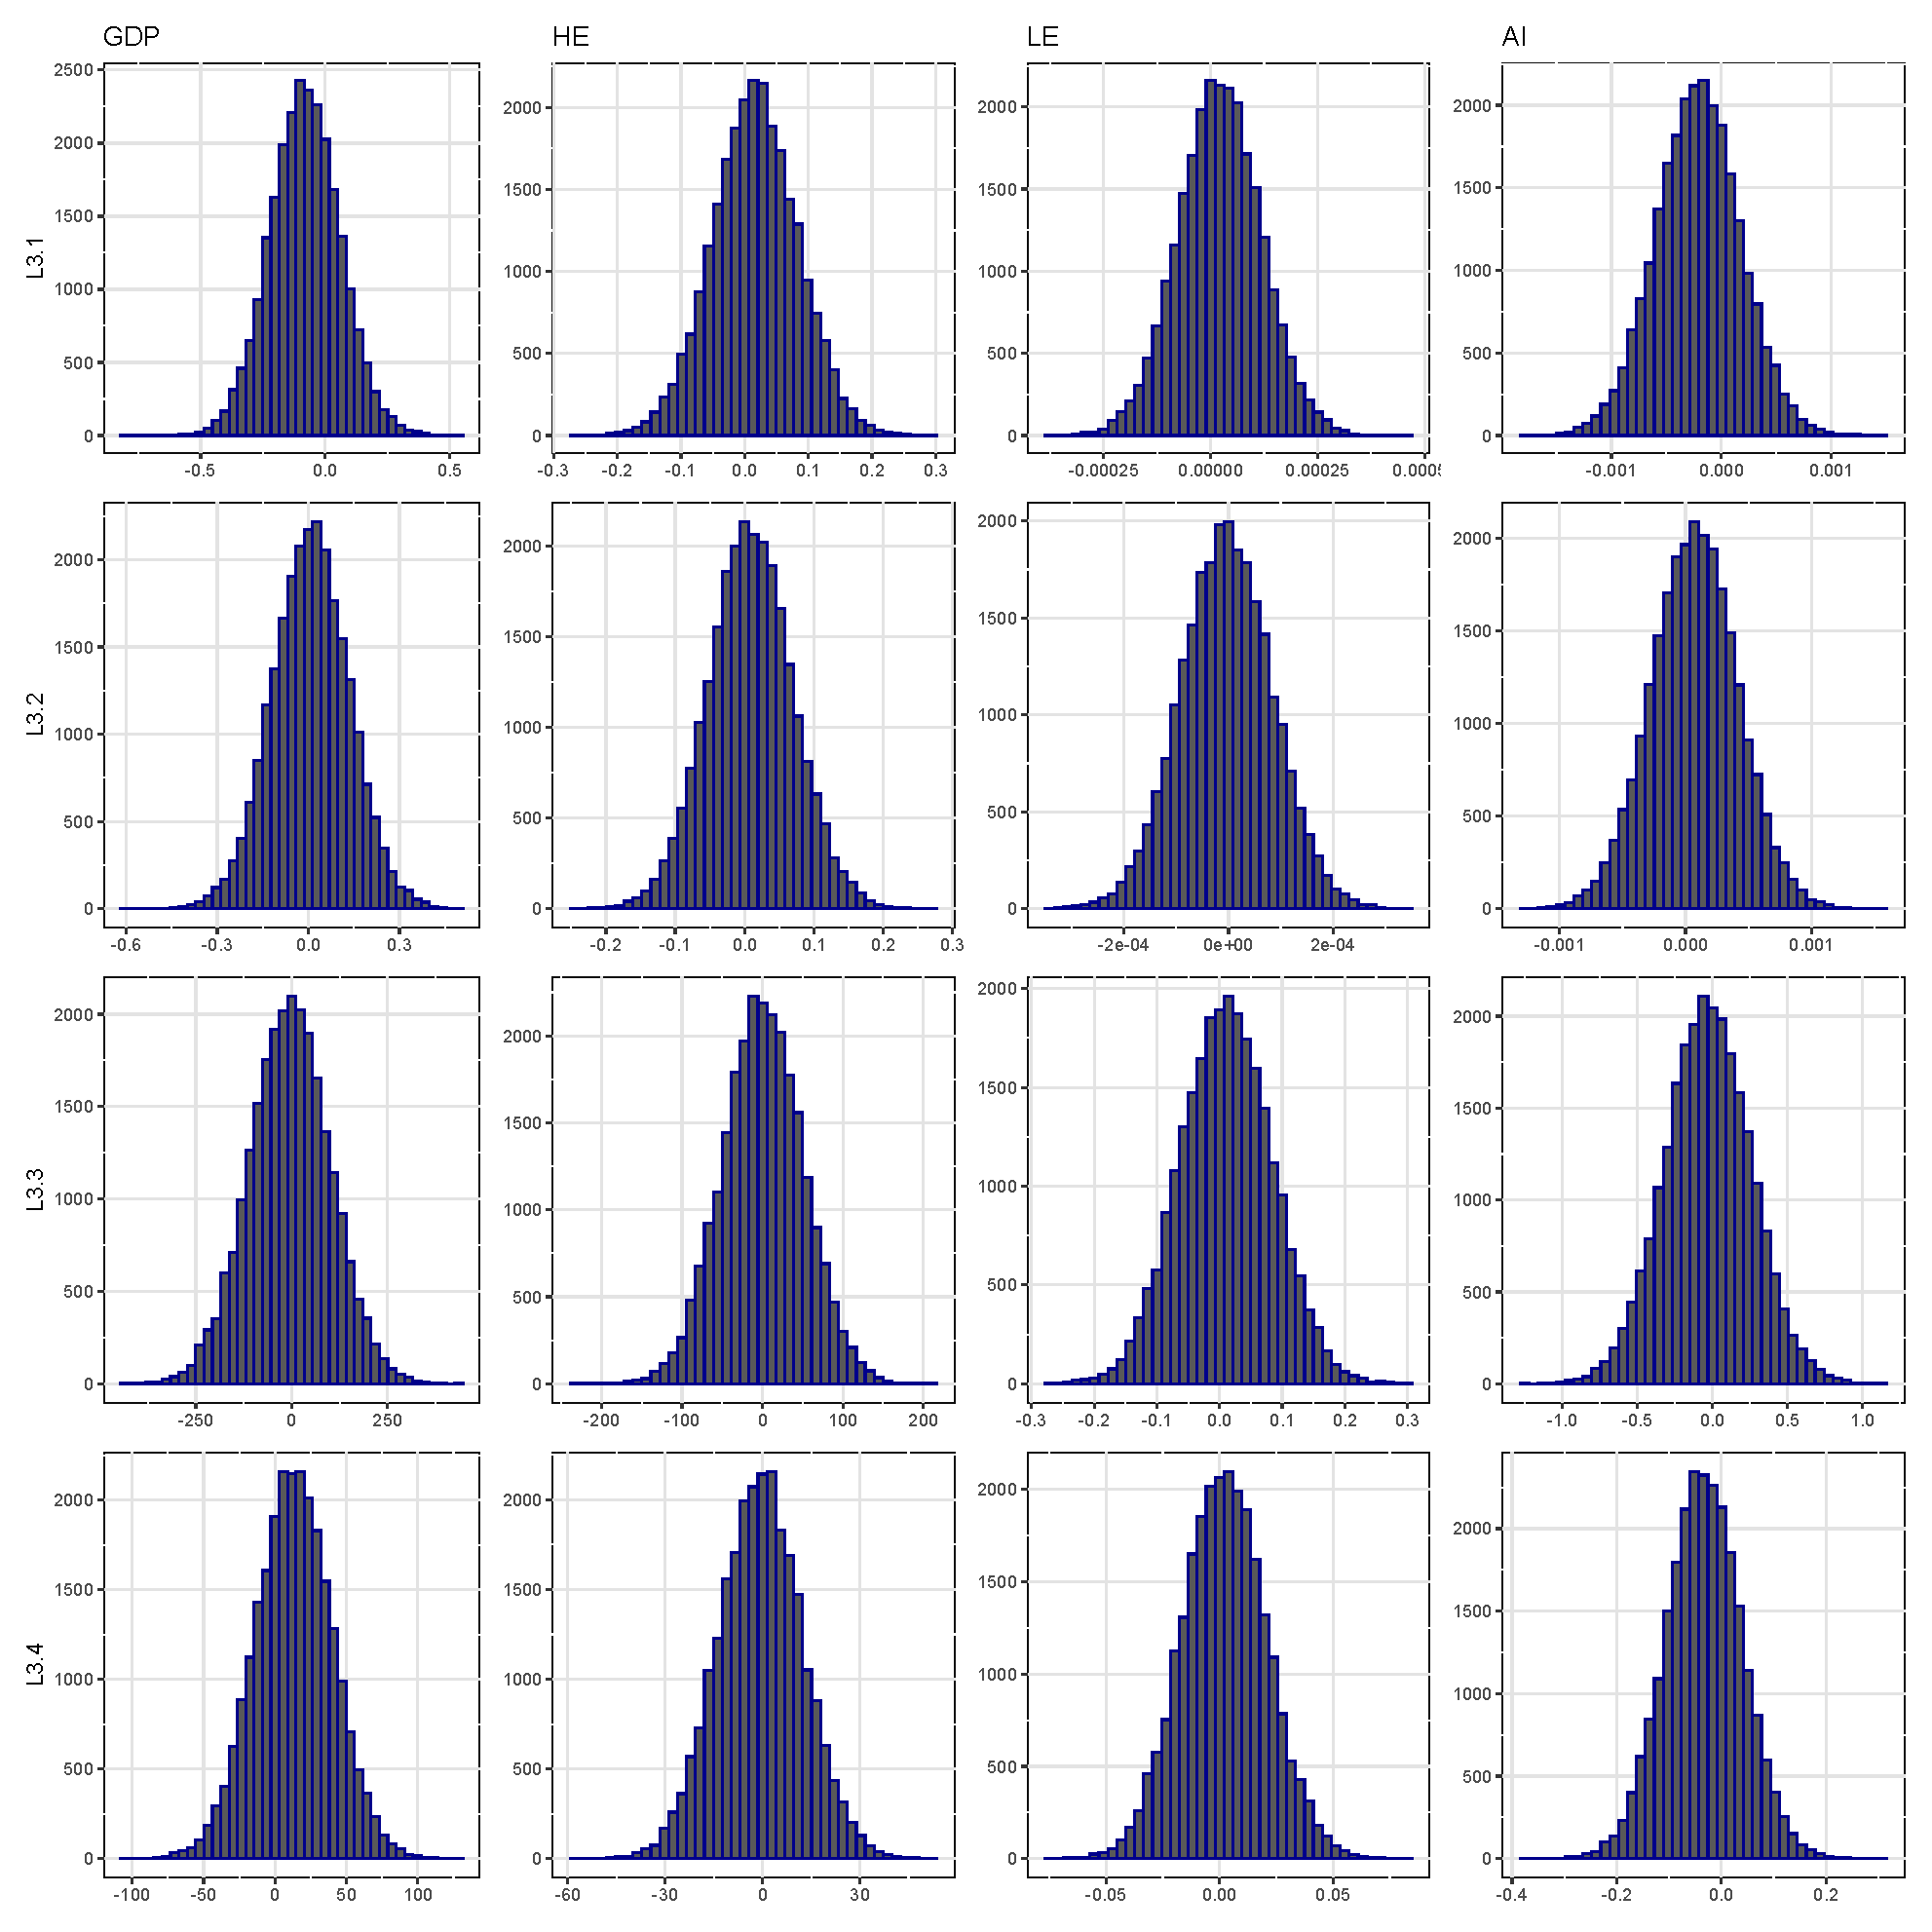
\includegraphics[width=\textwidth]{CoefLag3.eps}
    \end{subfigure}
        \caption{Conditional normal Inverse-Wishart prior: Estimated BVAR(3) coefficients' posterior distributions using Gibbs sampling.}
        \label{posterior_iw}
\end{figure}

\bibliography{Tex/ref}





\end{document}
